\chapter{Modelos Propuestos y Resultados} \label{Chapter:5}

Tal y como se ha comentado en la \autoref{Chapter:TransferLearning}, la explotación de las técnicas de transferencia de aprendizaje y por lo tanto el empleo de unos modelos con una serie de pesos ya definidos con respecto a un conjunto de datos determinado, constituyen la base de los sistemas propuestos en este capítulo.

\begin{figure}
    \centering
    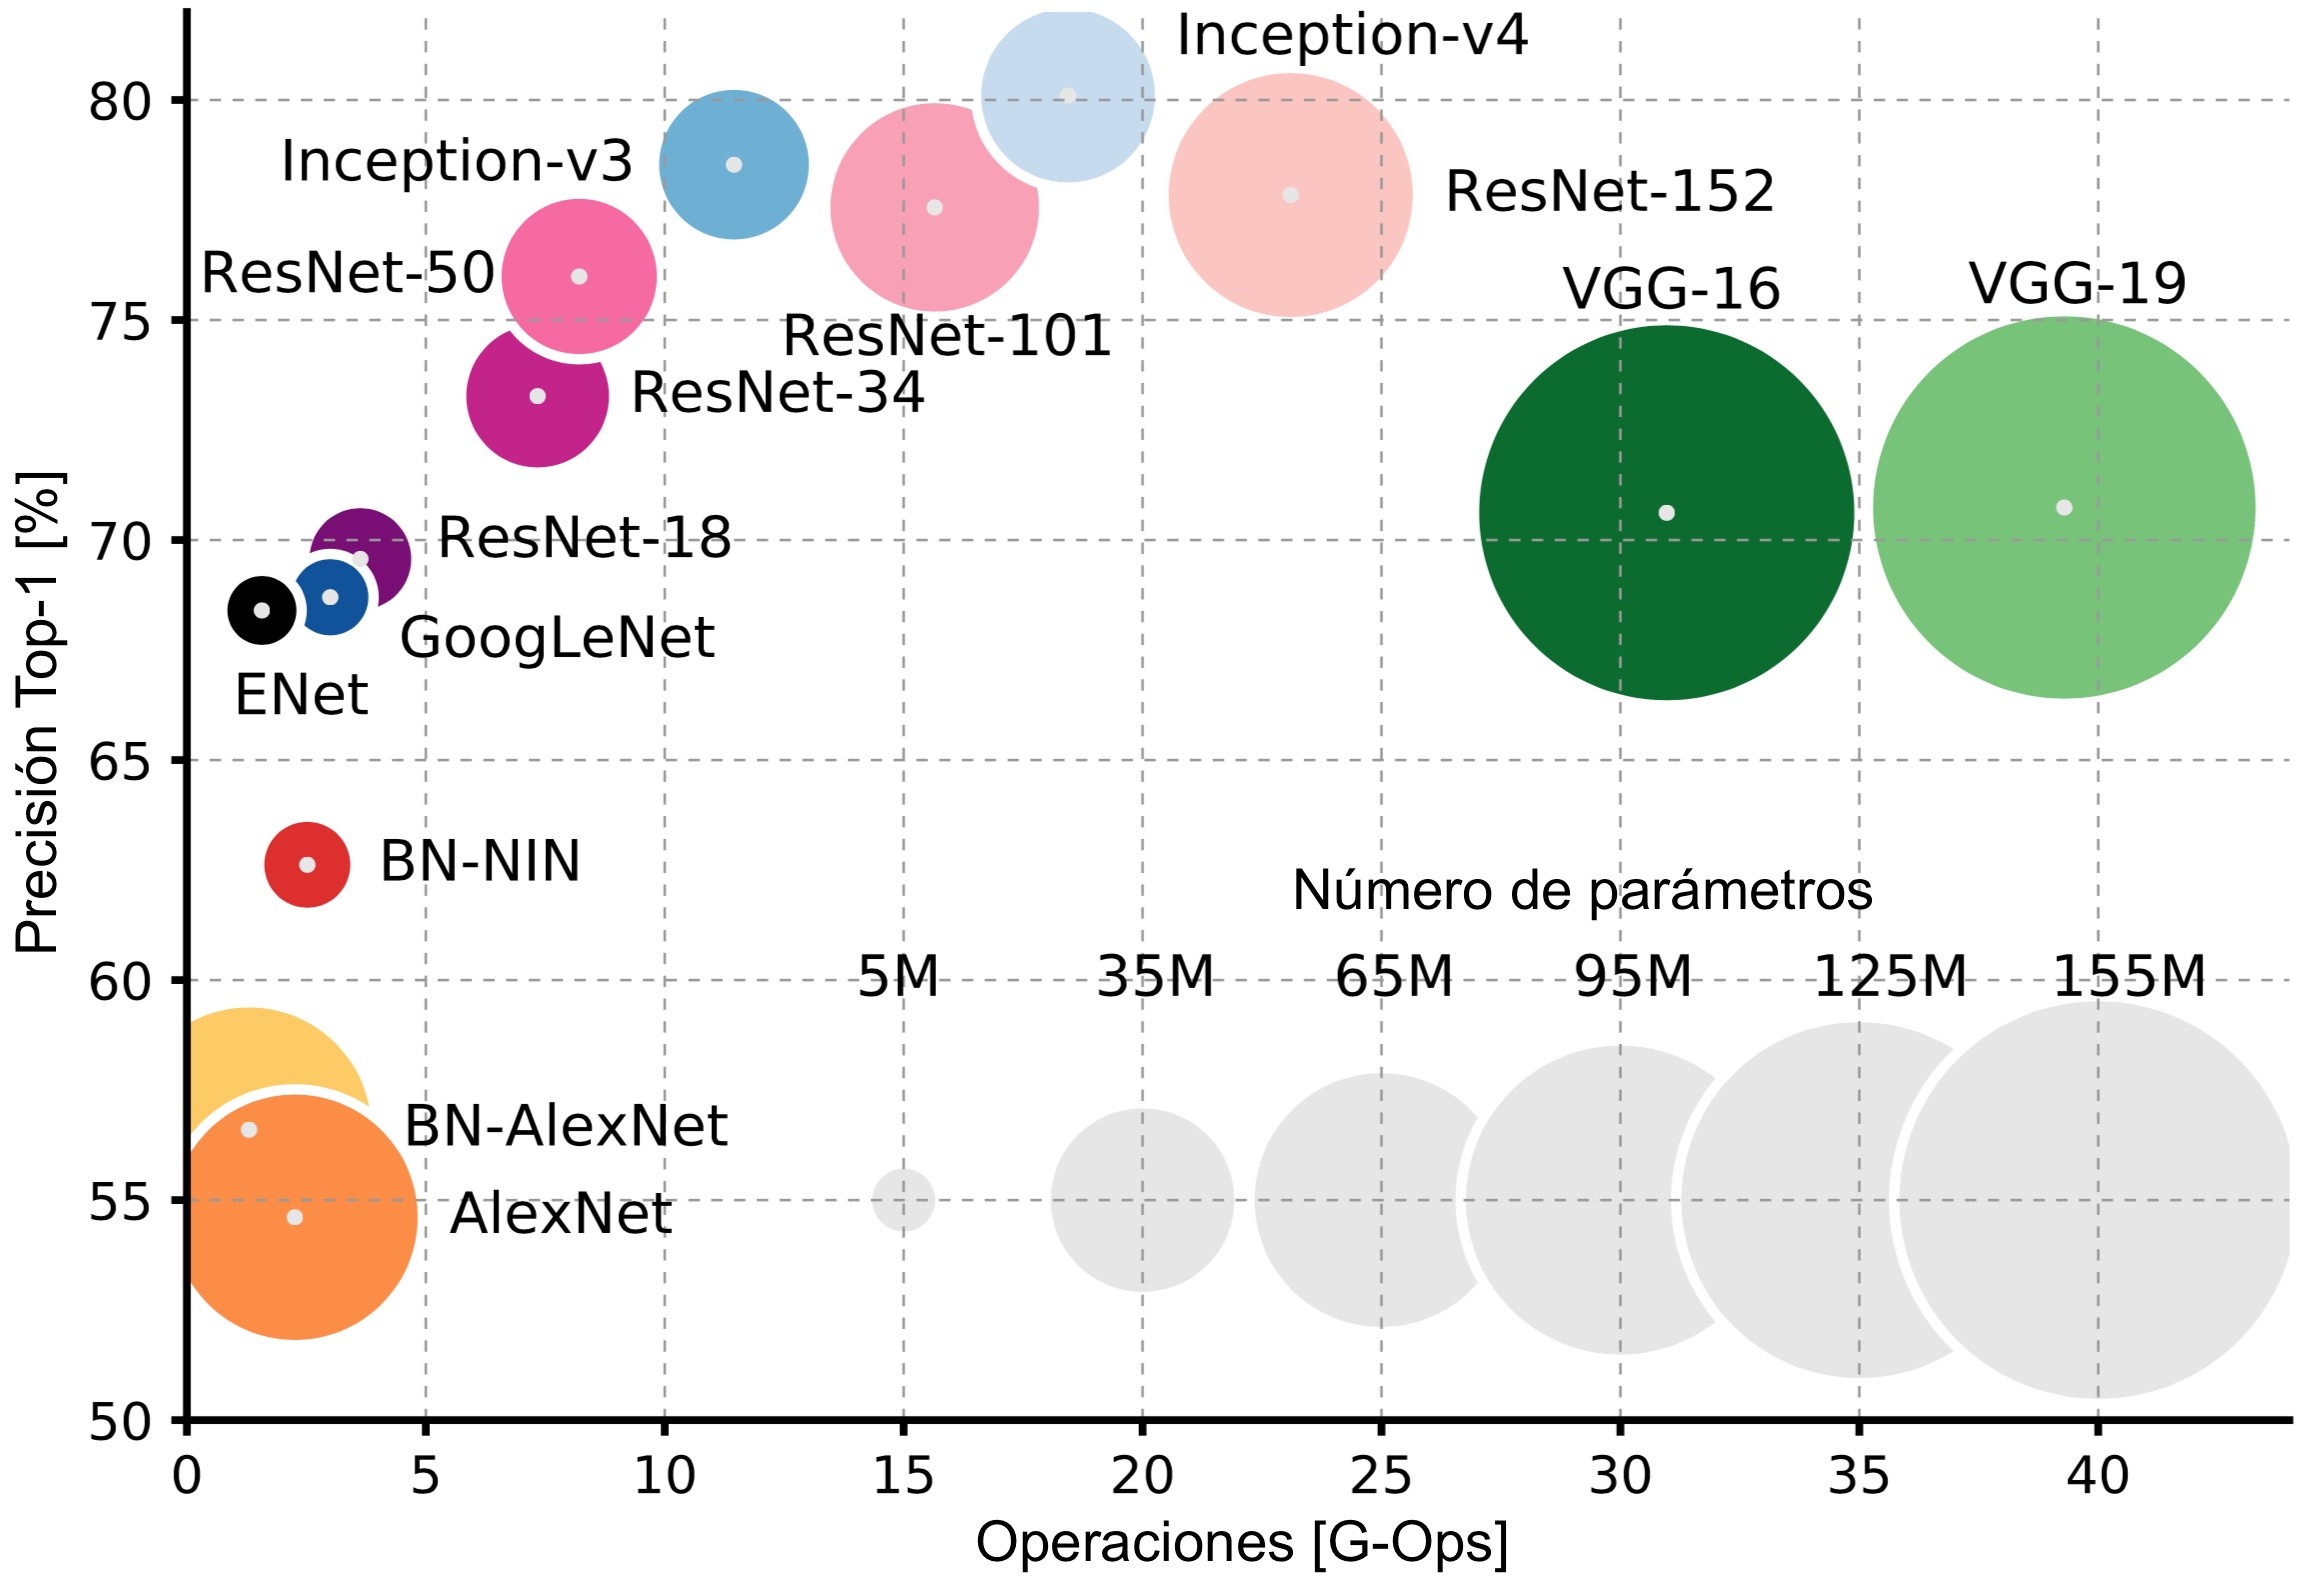
\includegraphics[scale=0.25]{Images/Models.png}
    \caption{Precisión Top-1 frente al coste computacional de una iteración del proceso de aprendizaje y el número de parámetros de la red \cite{Models}. Cabe destacar que aunque el modelo Inception-ResNet-v2 no se incluya en la figura, presenta características muy similares a Inception-v4 \cite{Inception-ResNet}.}
    \label{fig:Models}
\end{figure}

Por consiguiente, son utilizados en primera instancia los modelos Inception-v3 \cite{Inception-v3} e Inception-ResNet-v2 \cite{Inception-ResNet} con los pesos entrenados previamente sobre el conjunto de datos ImageNet descrito en la \autoref{Chapter:ImageNet}. Sin embargo, dado que las propiedades de las imágenes de esta base de datos difieren en gran medida de las características faciales que se intentan aprender y reconocer, se ha optado por explorar el uso de modelos menos eficaces pero enfocados al reconocimiento facial. Es por ello que en última instancia se emplea la arquitectura ResNet-50 \cite{ResNet} preetrenada con la base de datos VGGFace2 expuesta en la \autoref{Chapter:VGGFace2}. La comparación de estos modelos en el desempeño del desafío ILSVRC puede observarse en la \autoref{fig:Models}. Esta representación, además, escenifica la principal razón por la cual se han elegido estos sistemas concretos: son los que mejores tasas obtienen con respecto al coste computacional y al número de parámetros.

En definitiva, a lo largo del proceso de desarrollo de un sistema de reconocimiento de expresiones faciales válido, se han ido explorando numerosas arquitecturas (Inception-v3, Inception-ResNet-v2 y ResNet-50) y técnicas (aumento de datos) con el objetivo de ir obteniendo cada vez mejores resultados sobre la base de datos FER-2013. Asimismo, a fin de permitir una comparación justa con respecto a los resultados de la \autoref{Chapter:RelatedWork}, son utilizados los protocolos de uso estipulados inicialmente por este desafío y que establecen la división de esta base de datos en tres conjuntos diferentes: entrenamiento, validación y evaluación.

\section{Arquitecturas afinadas}

\subsection{Inception-v3} \label{Chapter:ArchitectureInceptionV3}

Inception-v3 es el resultado de las investigaciones llevadas a cabo por el equipo de Google para conseguir un modelo con una arquitectura cada vez más profunda e inteligente y capaz de desenvolverse de forma eficiente, tanto computacionalmente como cualitativamente, en el desafío ILSVR.

\begin{figure}
    \centering
    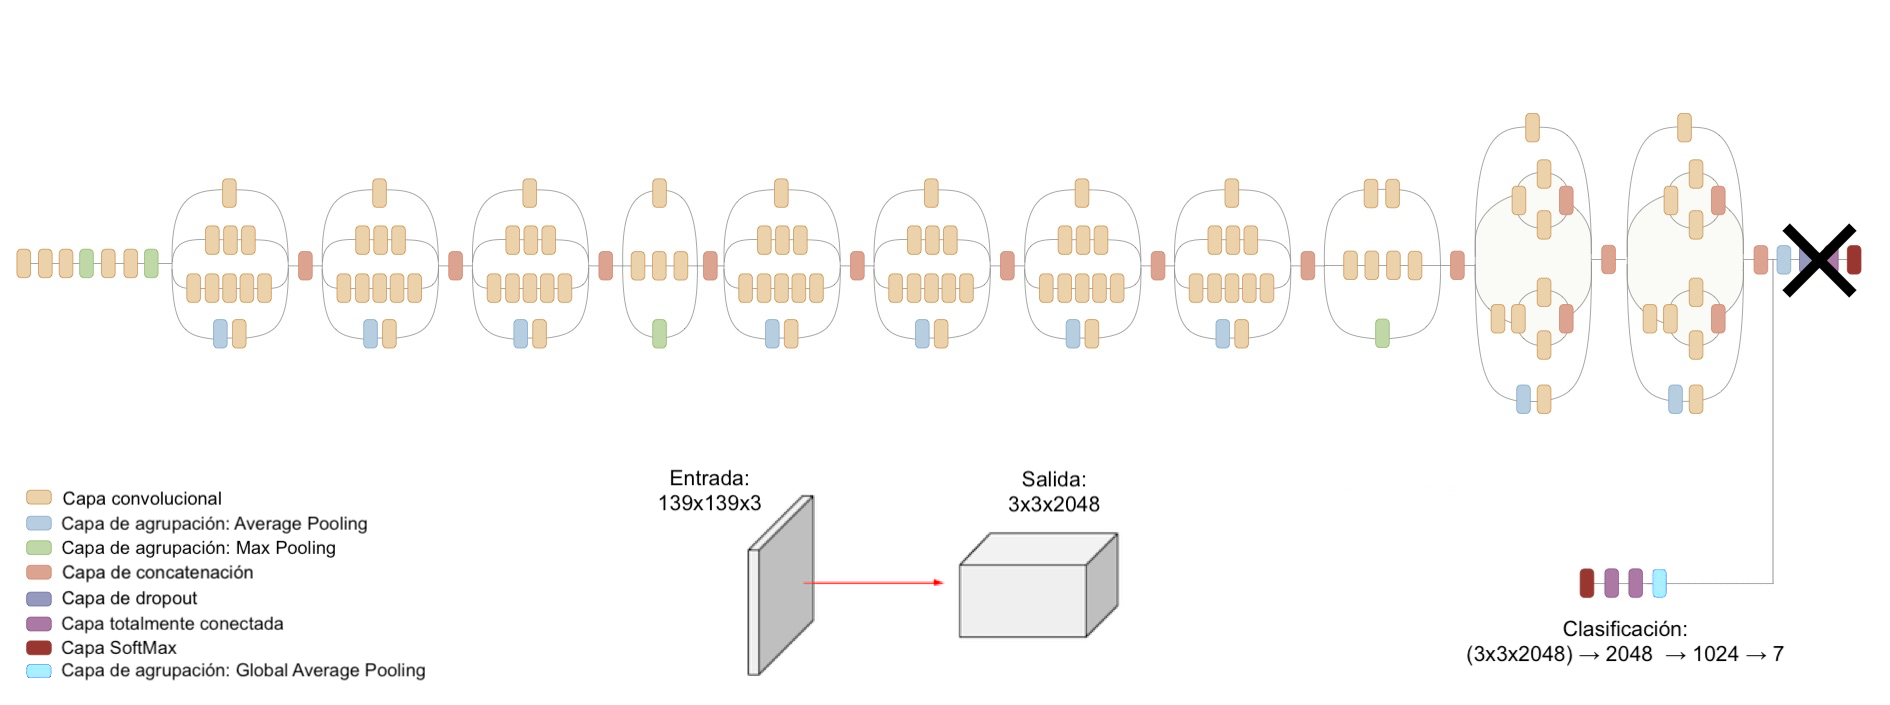
\includegraphics[width=\textwidth]{Images/Inception-v3.png}
    \caption{Arquitectura del modelo Inception-v3 adaptada al problema del reconocimiento de expresiones faciales \cite{img:Inception-v3}.}
    \label{fig:Inception-v3}
\end{figure}

\begin{figure}
    \centering
    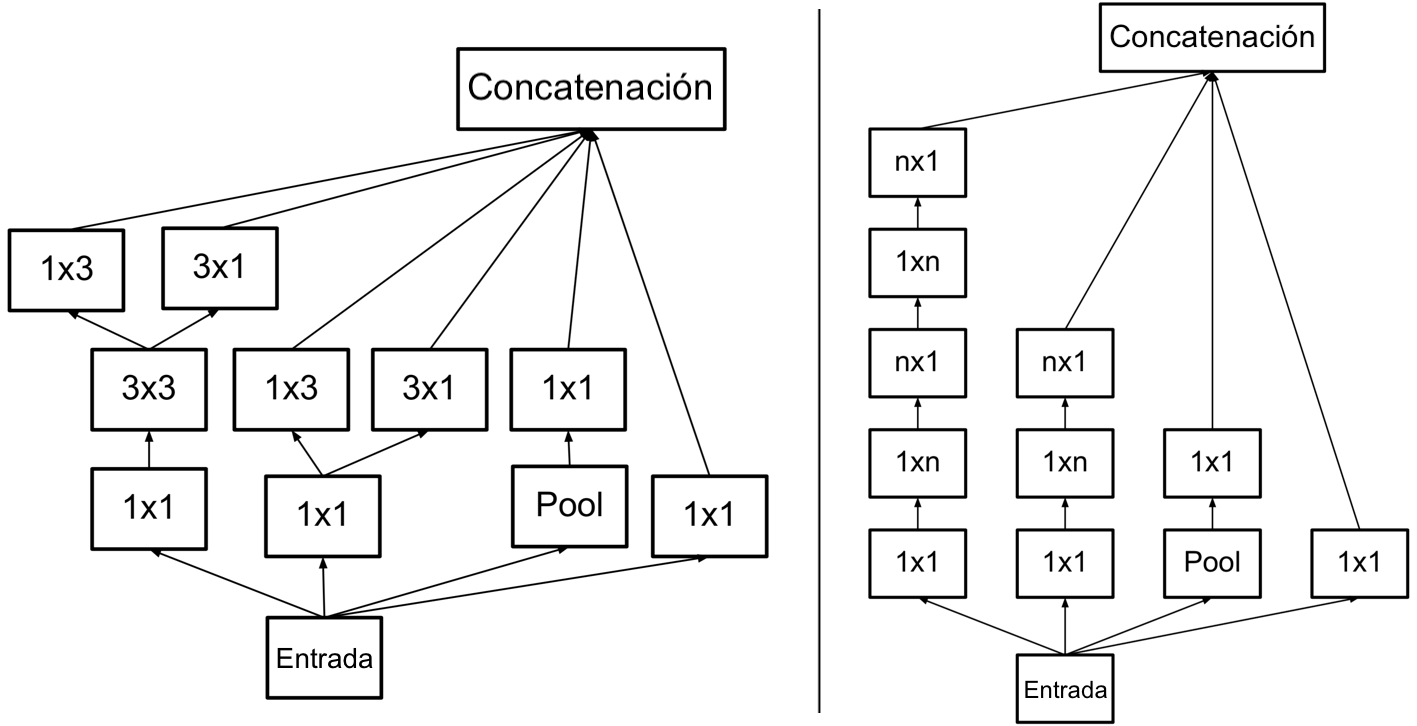
\includegraphics[width=\textwidth]{Images/InceptionModules.png}
    \caption{Módulos Inception empleados en la arquitectura Inception-v3. Estos bloques son utilizados para promover las representaciones de alta dimensión (izquierda) y la factorización de las convoluciones de dimensión $n\times n$ (derecha) \cite{Inception-v3}.}
    \label{fig:InceptionModules}
\end{figure}

En la \autoref{fig:Inception-v3} se muestra la estructura simplificada y adaptada al problema del reconocimiento de expresiones faciales del modelo Inception-v3. Esta arquitectura propuesta es básicamente una sucesión de tramos convolucionales y no linealidades, empleándose la función de activación ReLU y la normalización por lotes en cada una de las etapas según lo descrito en \autoref{Chapter:Layers}, aunque esto último no se muestre explícitamente en la representación anteriormente mencionada. Como se ha podido advertir, la característica principal de este modelo es el hecho de que el flujo de datos a lo largo de algunas secciones de esta red no es secuencial, sino que se realiza en paralelo. Estas agrupaciones son conocidas como módulos Inception y representan la solución a los problemas de eficiencia de las redes estado del arte predecesoras, cumpliendo, además, la misma función y obteniendo los mismos resultados que una capa convolucional estándar. Las diferentes estructuras de estos módulos empleados por el modelo Inception-v3 pueden observarse en la \autoref{fig:InceptionModules}. La idea detrás de estas disposiciones paralelas es que dada la misma entrada para varias capas convolucionales o de agrupación de distinto tamaño se generen características únicas para cada una de ellas que posteriormente procederán a concatenarse. Este enfoque, sin embargo, da lugar a una salida con una profundidad extremadamente grande que es solucionada mediante la utilización de filtros convolucionales $1\times 1$, especialmente efectivos para reducir la dimensionalidad \cite{NetworkInNetwork} e incorporados justo antes de las capas convolucionales de mayor tamaño. Otro de los puntos que es explotado por los módulos Inception es la sustitución de los filtros tradicionales de tamaño $n\times n$ por una secuencia de capas convolucionales de dimensiones $1\times n$ y $n \times 1$. Mediante esta técnica se consigue disminuir drásticamente los costes computacionales a medida que $n$ aumenta. En la práctica y tal como se ha visto en la \autoref{fig:InceptionModules}, son utilizados básicamente filtros con $n = 7$ y $n = 3$.

Por otro lado, dado que esta red ha sido diseñada para competir en el reto ImageNet, es necesario modificar la etapa de clasificación del modelo Inception-v3 original, tal y como se ha indicado en la \autoref{fig:Inception-v3}. De esta forma, en primer lugar se ha procedido a introducir una capa basada en la agrupación promedio global, que impone la correspondencia entre los mapas de activación y las clases, reduce el número de parámetros y además es menos propensa al sobreaprendizaje que las capas convencionales totalmente conectadas \cite{NetworkInNetwork}. Posteriormente y con la finalidad de reducir la dimensionalidad de la red de una manera suave a las 7 clases correspondientes a las expresiones faciales que se pretenden clasificar, son insertadas dos capas totalmente conectadas de 2\,048 y 1\,024 neuronas respectivamente.

En cuanto a la entrada y puesto que las imágenes del conjunto de datos FER-2013 presentan una resolución bastante baja ($48\times 48$ píxeles) en comparación con las representaciones de ImageNet ($299\times 299$ píxeles) y las mínimas aceptadas por el modelo Inception-v3 ($139\times 139$ píxeles), es requerida una modificación parcial del comportamiento de la primera etapa de la arquitectura utilizada. Concretamente es necesario modificar las dos primeras capas de agrupación para evitar la omisión de parte de los datos inyectados en la entrada. Sin embargo, esto ya es realizado por Keras de forma automática.

\subsection{Inception-ResNet-v2}

Inception-ResNet-v2 es una ampliación, llevada a cabo por el grupo de inteligencia artificial de Google, de los conceptos planteados en la arquitectura Inception-v3 mediante dos metodologías que tienen como fin aumentar el rendimiento y el número de módulos Inception. La primera consiste simplemente en el empleo de una estructura ligeramente distinta dentro de los propios bloques en función de la posición de éstos en la red, mientras que la segunda, por su parte, plantea la utilización de conexiones residuales, similares a las desarrolladas por el equipo de Microsoft en las redes ResNet \cite{ResNet}, para acelerar el proceso de entrenamiento y aumentar la profundidad de la arquitectura. Estas conexiones, además, favorecen la simplificación de los bloques Inception. En definitiva, estas dos ideas permiten alcanzar e incluso superar el rendimiento de los modelos puros de Inception con un número significativamente menor de iteraciones de entrenamiento.

\begin{figure}
    \centering
    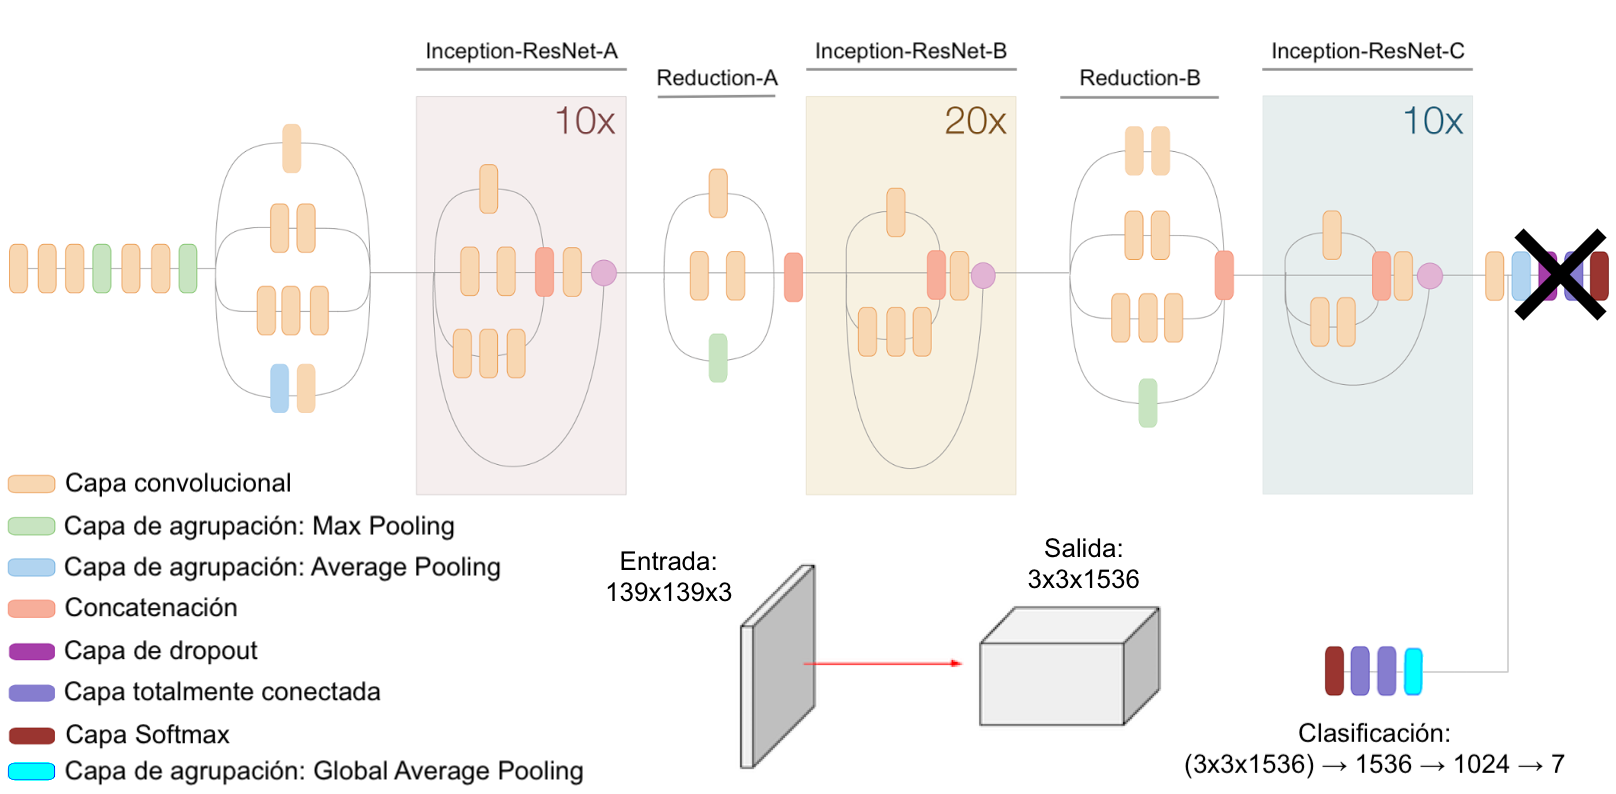
\includegraphics[width=\textwidth]{Images/Inception-ResNet-v2.png}
    \caption{Arquitectura comprimida y adaptada al problema del reconocimiento de expresiones del modelo Inception-ResNet-v2 \cite{img:Inception-ResNet-v2}.}
    \label{fig:Inception-ResNet-v2}
\end{figure}

\begin{figure}
    \centering
    \begin{subfigure}[t]{.45\textwidth}
      \centering
      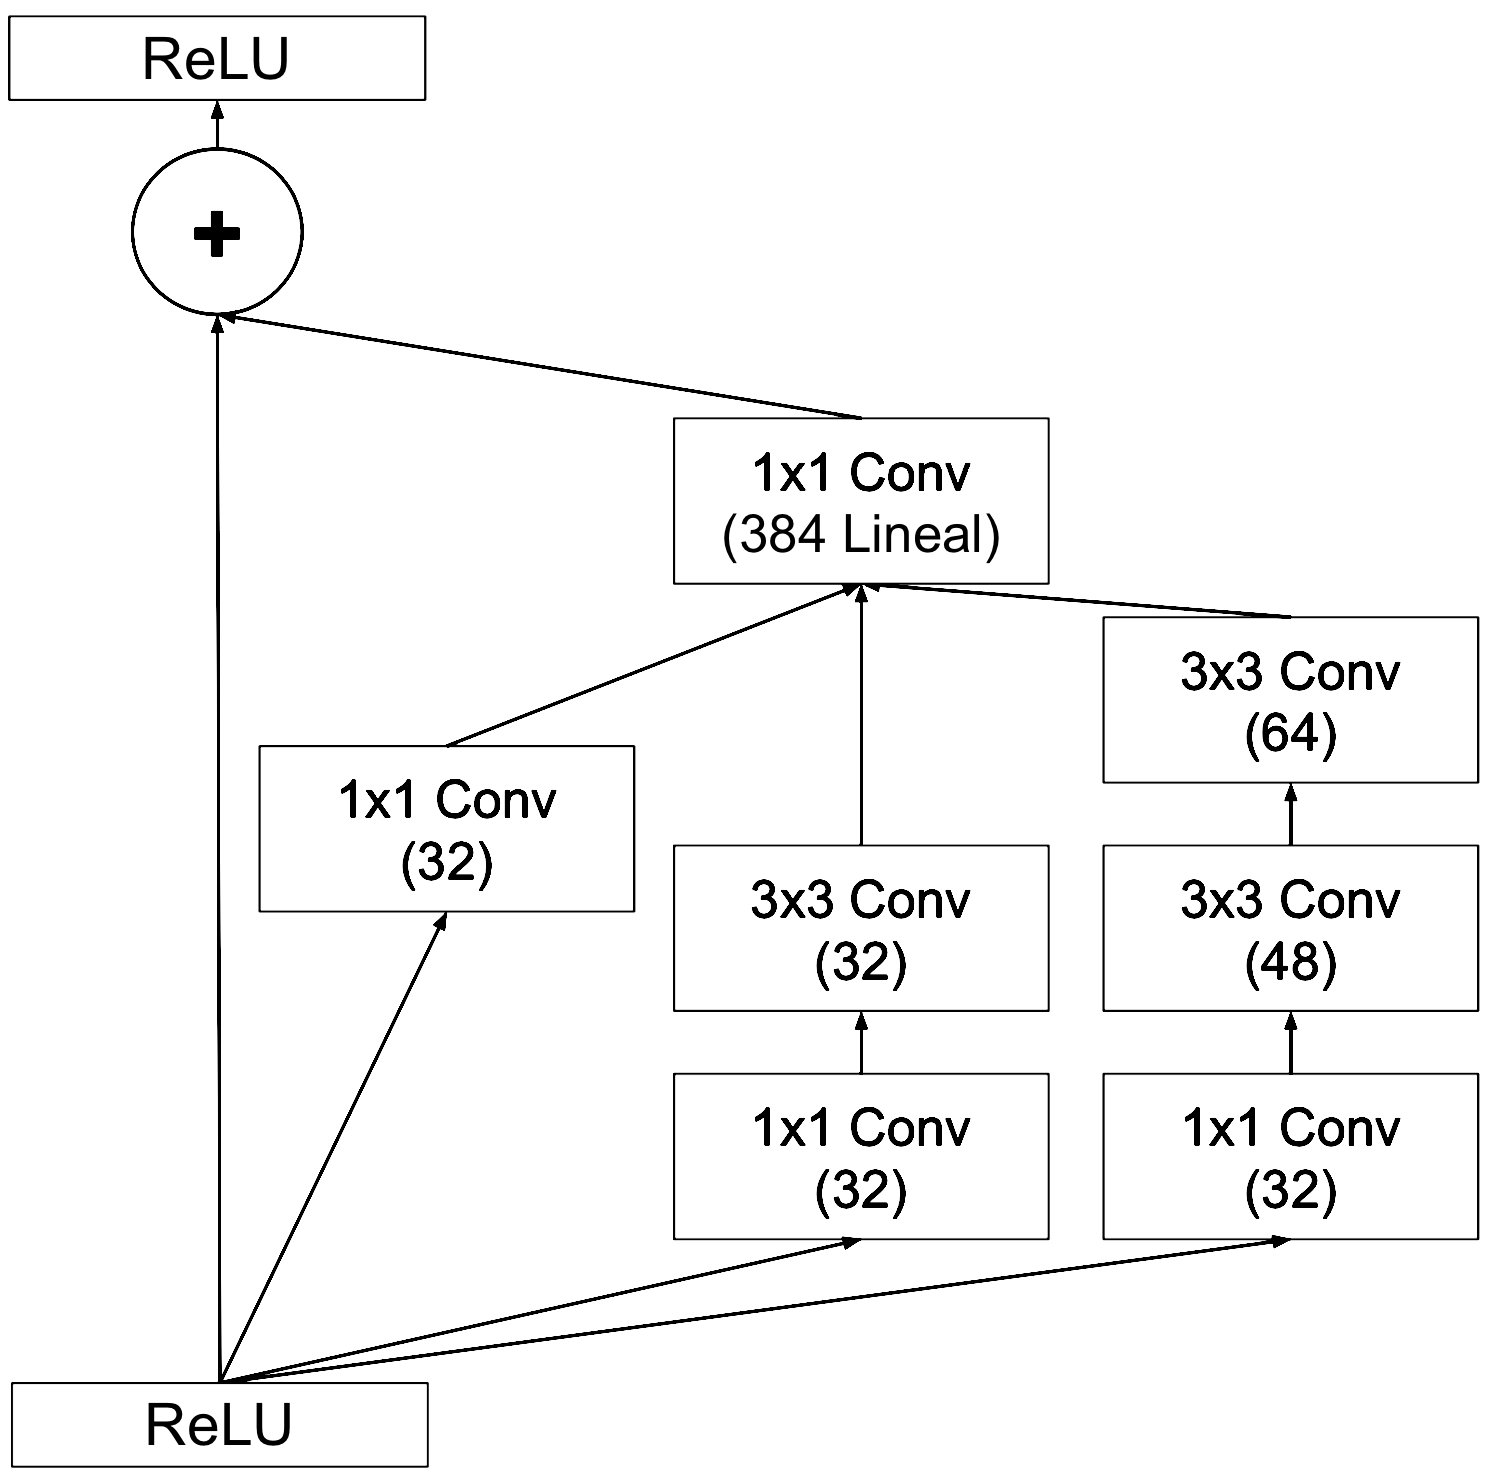
\includegraphics[width=.8\linewidth]{Images/Inception-ResNet-A.png}
      \caption{Bloque Inception-ResNet-A.}
      \label{fig:Inception-ResNet-A}
    \end{subfigure}
    \hfill
    \begin{subfigure}[t]{.45\textwidth}
      \centering
      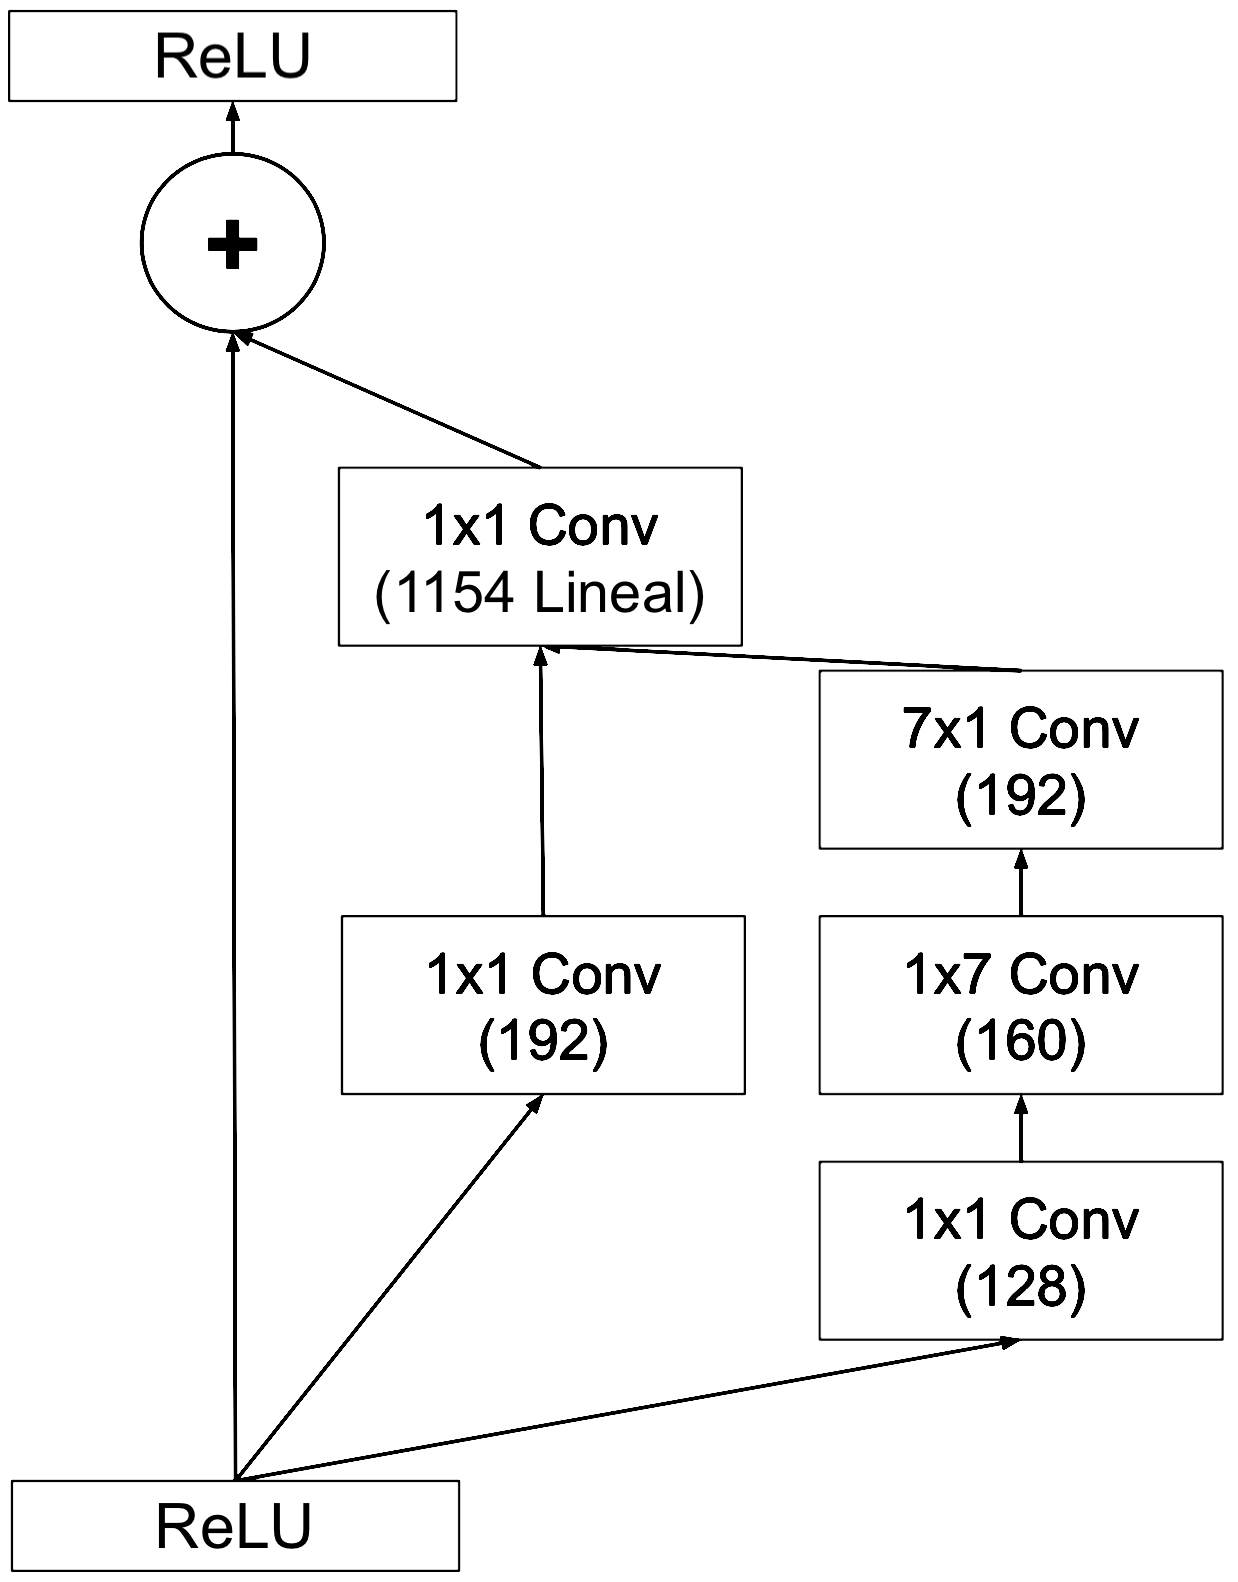
\includegraphics[width=.8\linewidth]{Images/Inception-ResNet-B.png}
      \caption{Bloque Inception-ResNet-B.}
      \label{fig:Inception-ResNet-B}
    \end{subfigure}
    
    \vspace{1cm}
    \begin{subfigure}[t]{.45\textwidth}
      \centering
      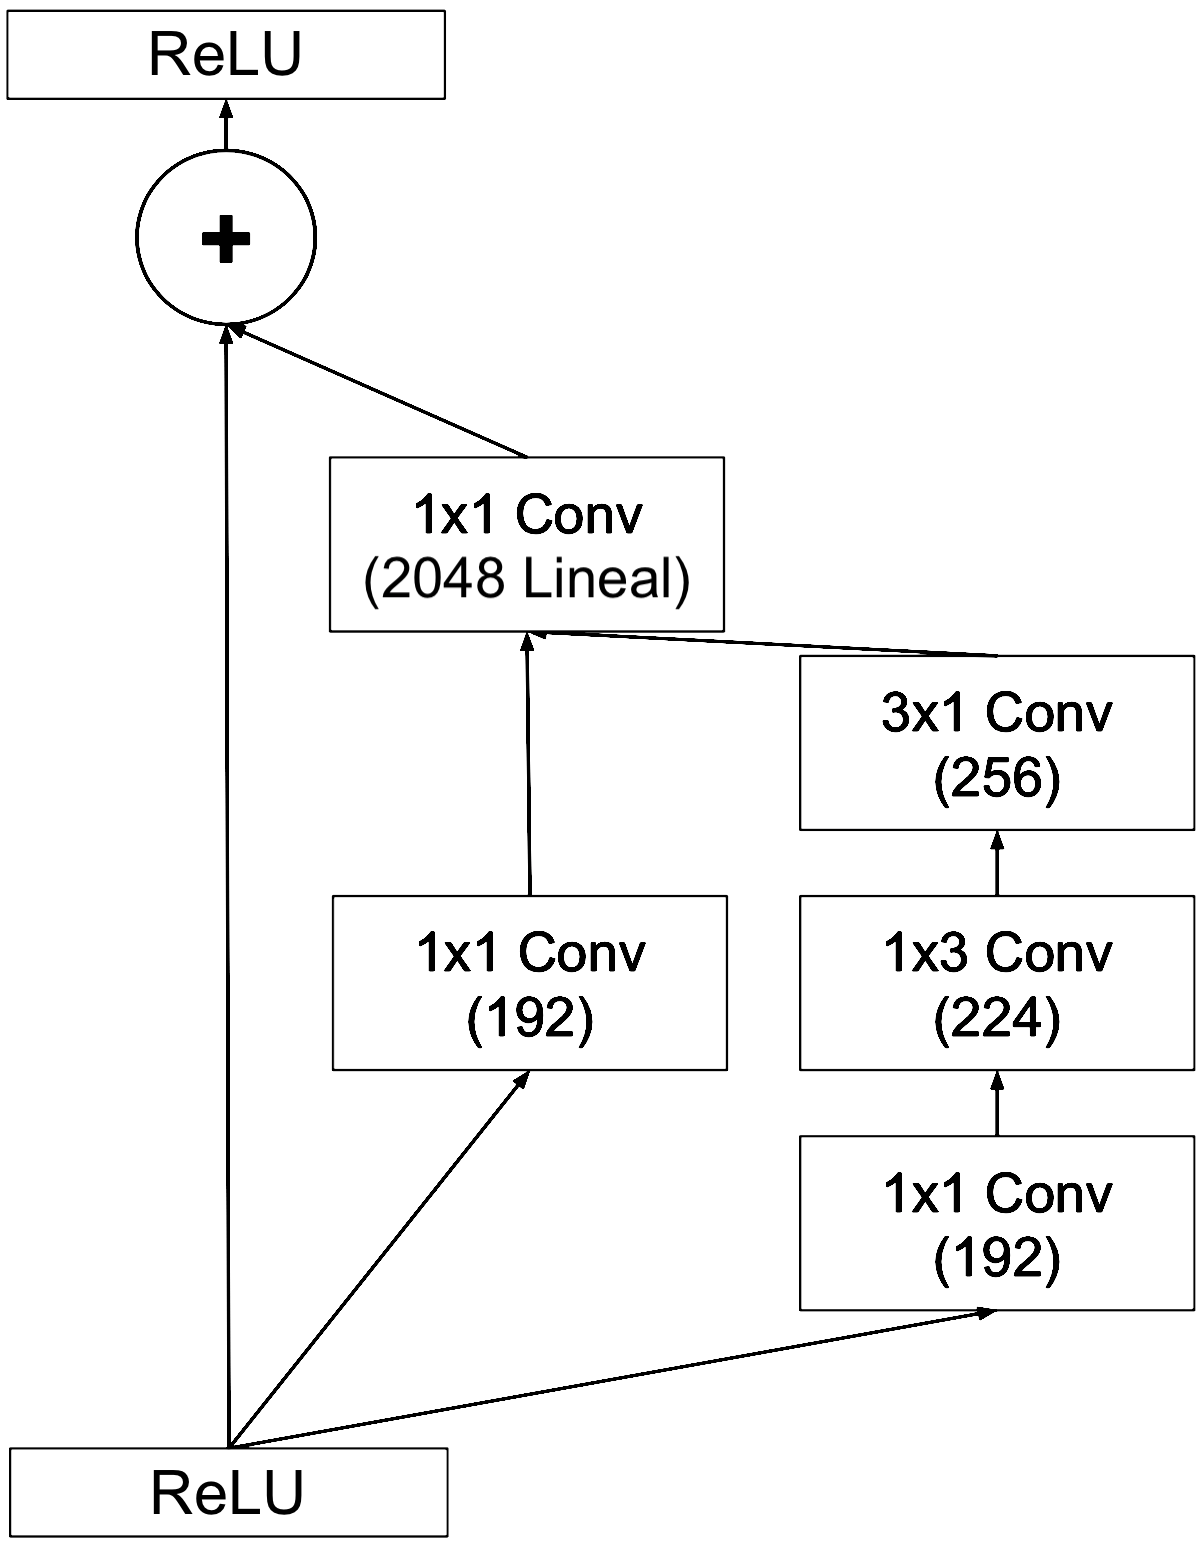
\includegraphics[width=.7\linewidth]{Images/Inception-ResNet-C.png}
      \caption{Bloque Inception-ResNet-C.}
      \label{fig:Inception-ResNet-C}
    \end{subfigure}
    
    \vspace{1cm}
    \begin{subfigure}[t]{.45\textwidth}
      \centering
      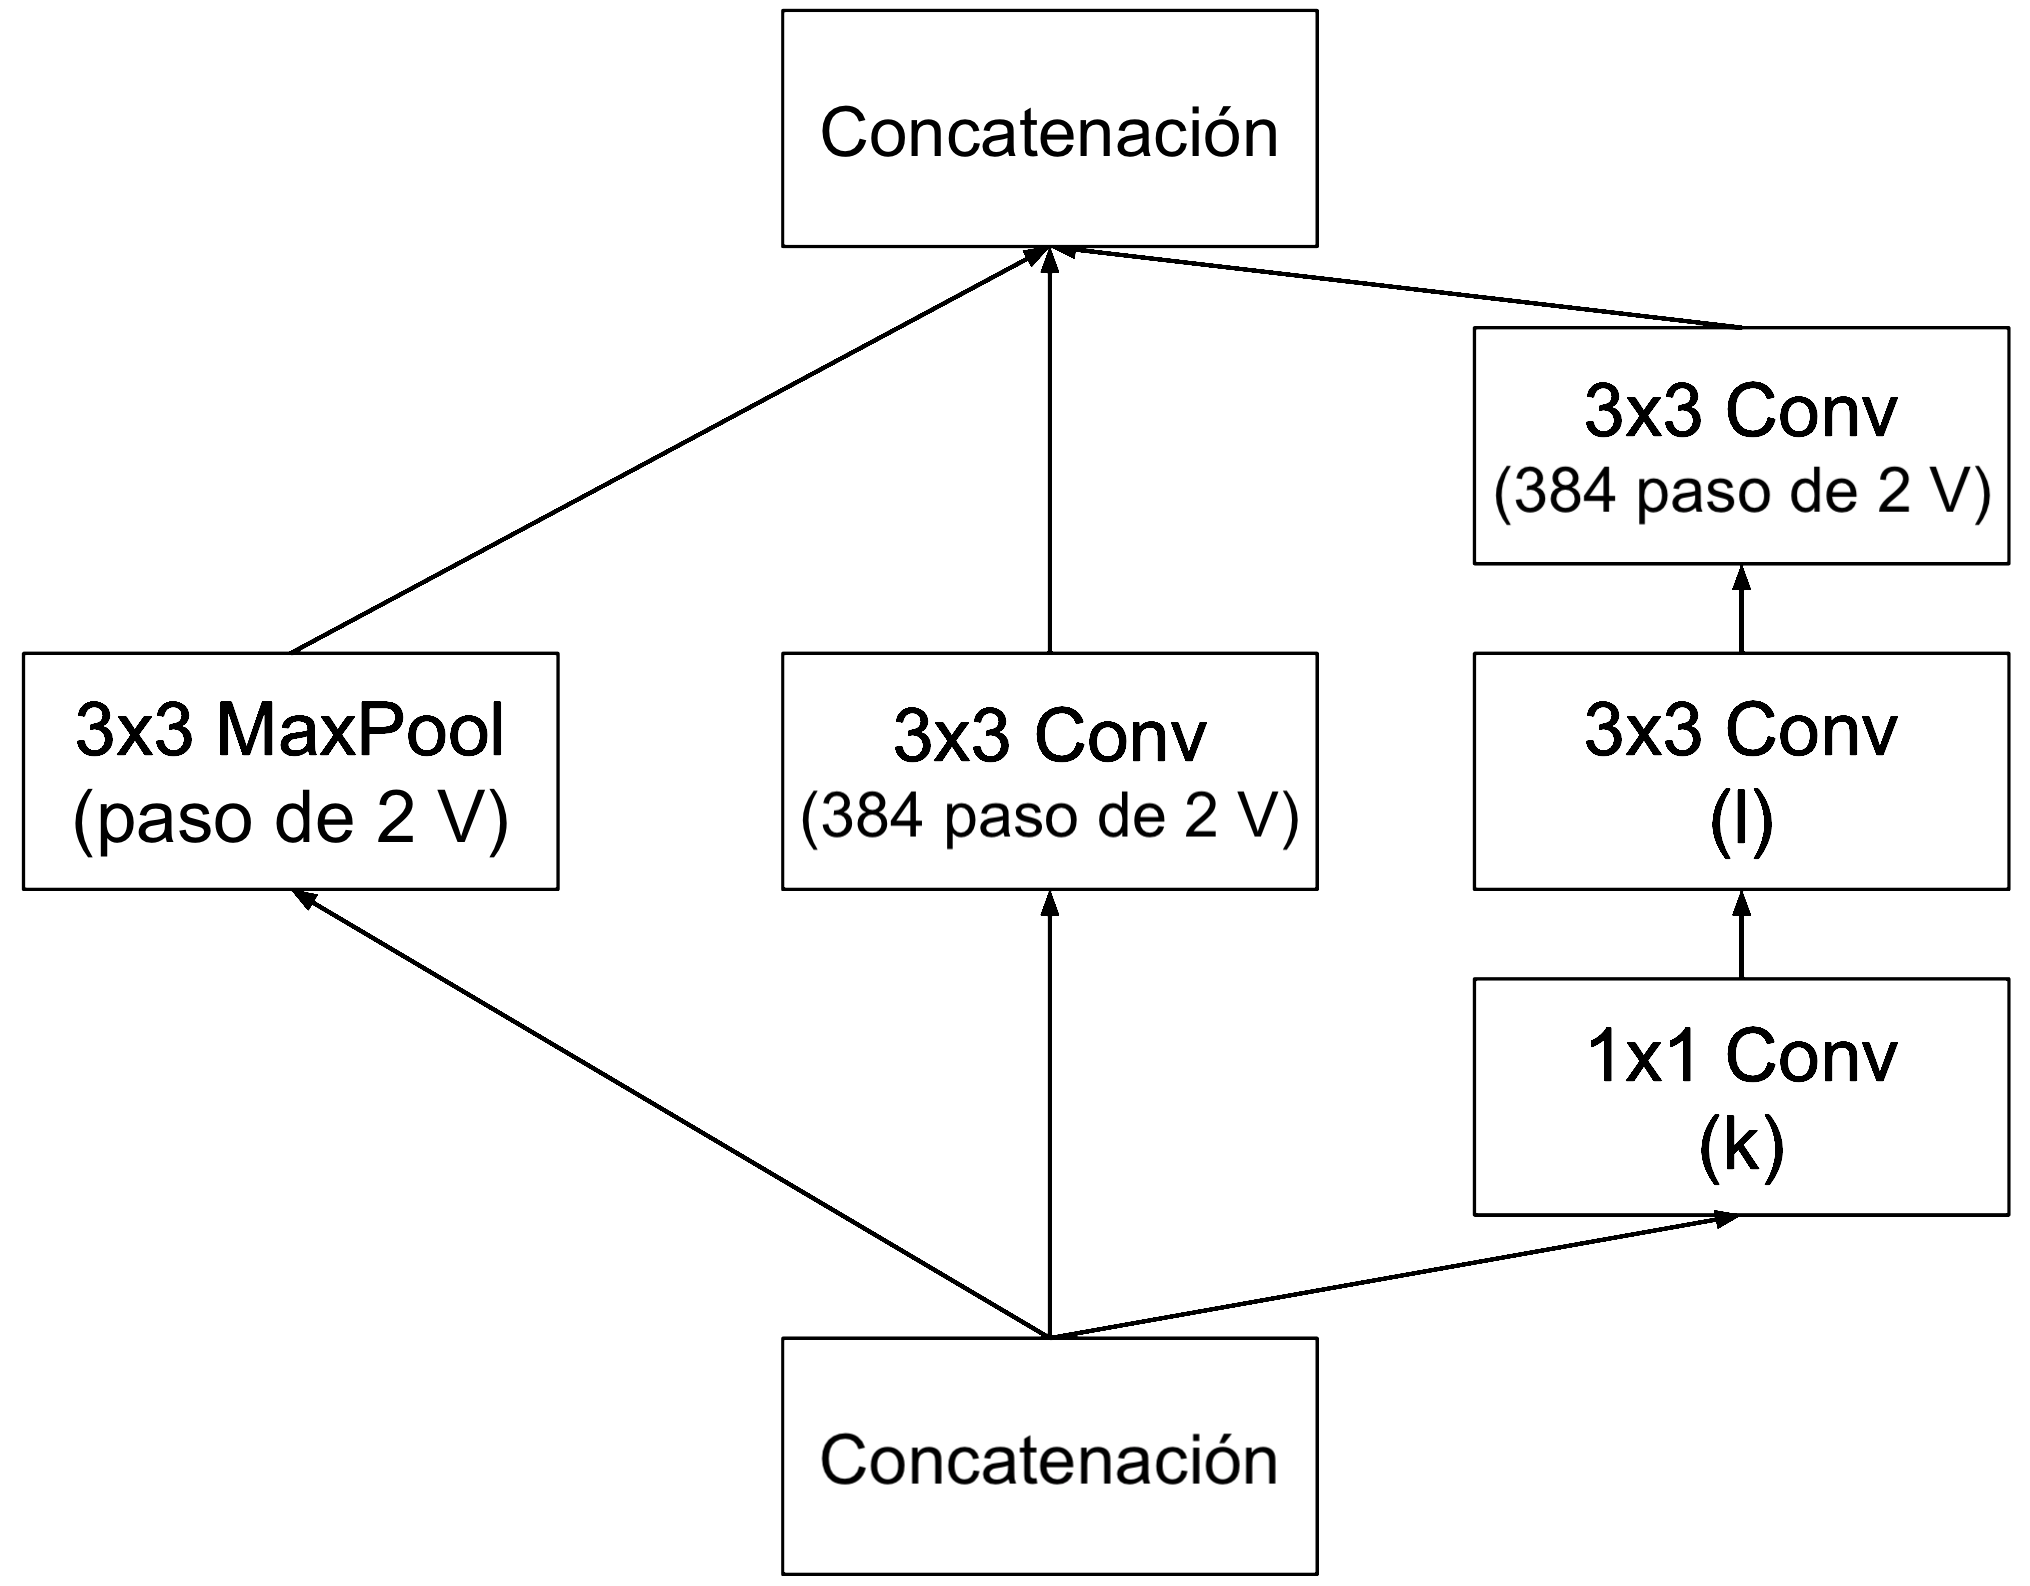
\includegraphics[width=.9\linewidth]{Images/Reduction-A.png}
      \caption{Bloque Reduction-A.}
      \label{fig:Reduction-A}
    \end{subfigure}
    \hfill
    \begin{subfigure}[t]{.45\textwidth}
      \centering
      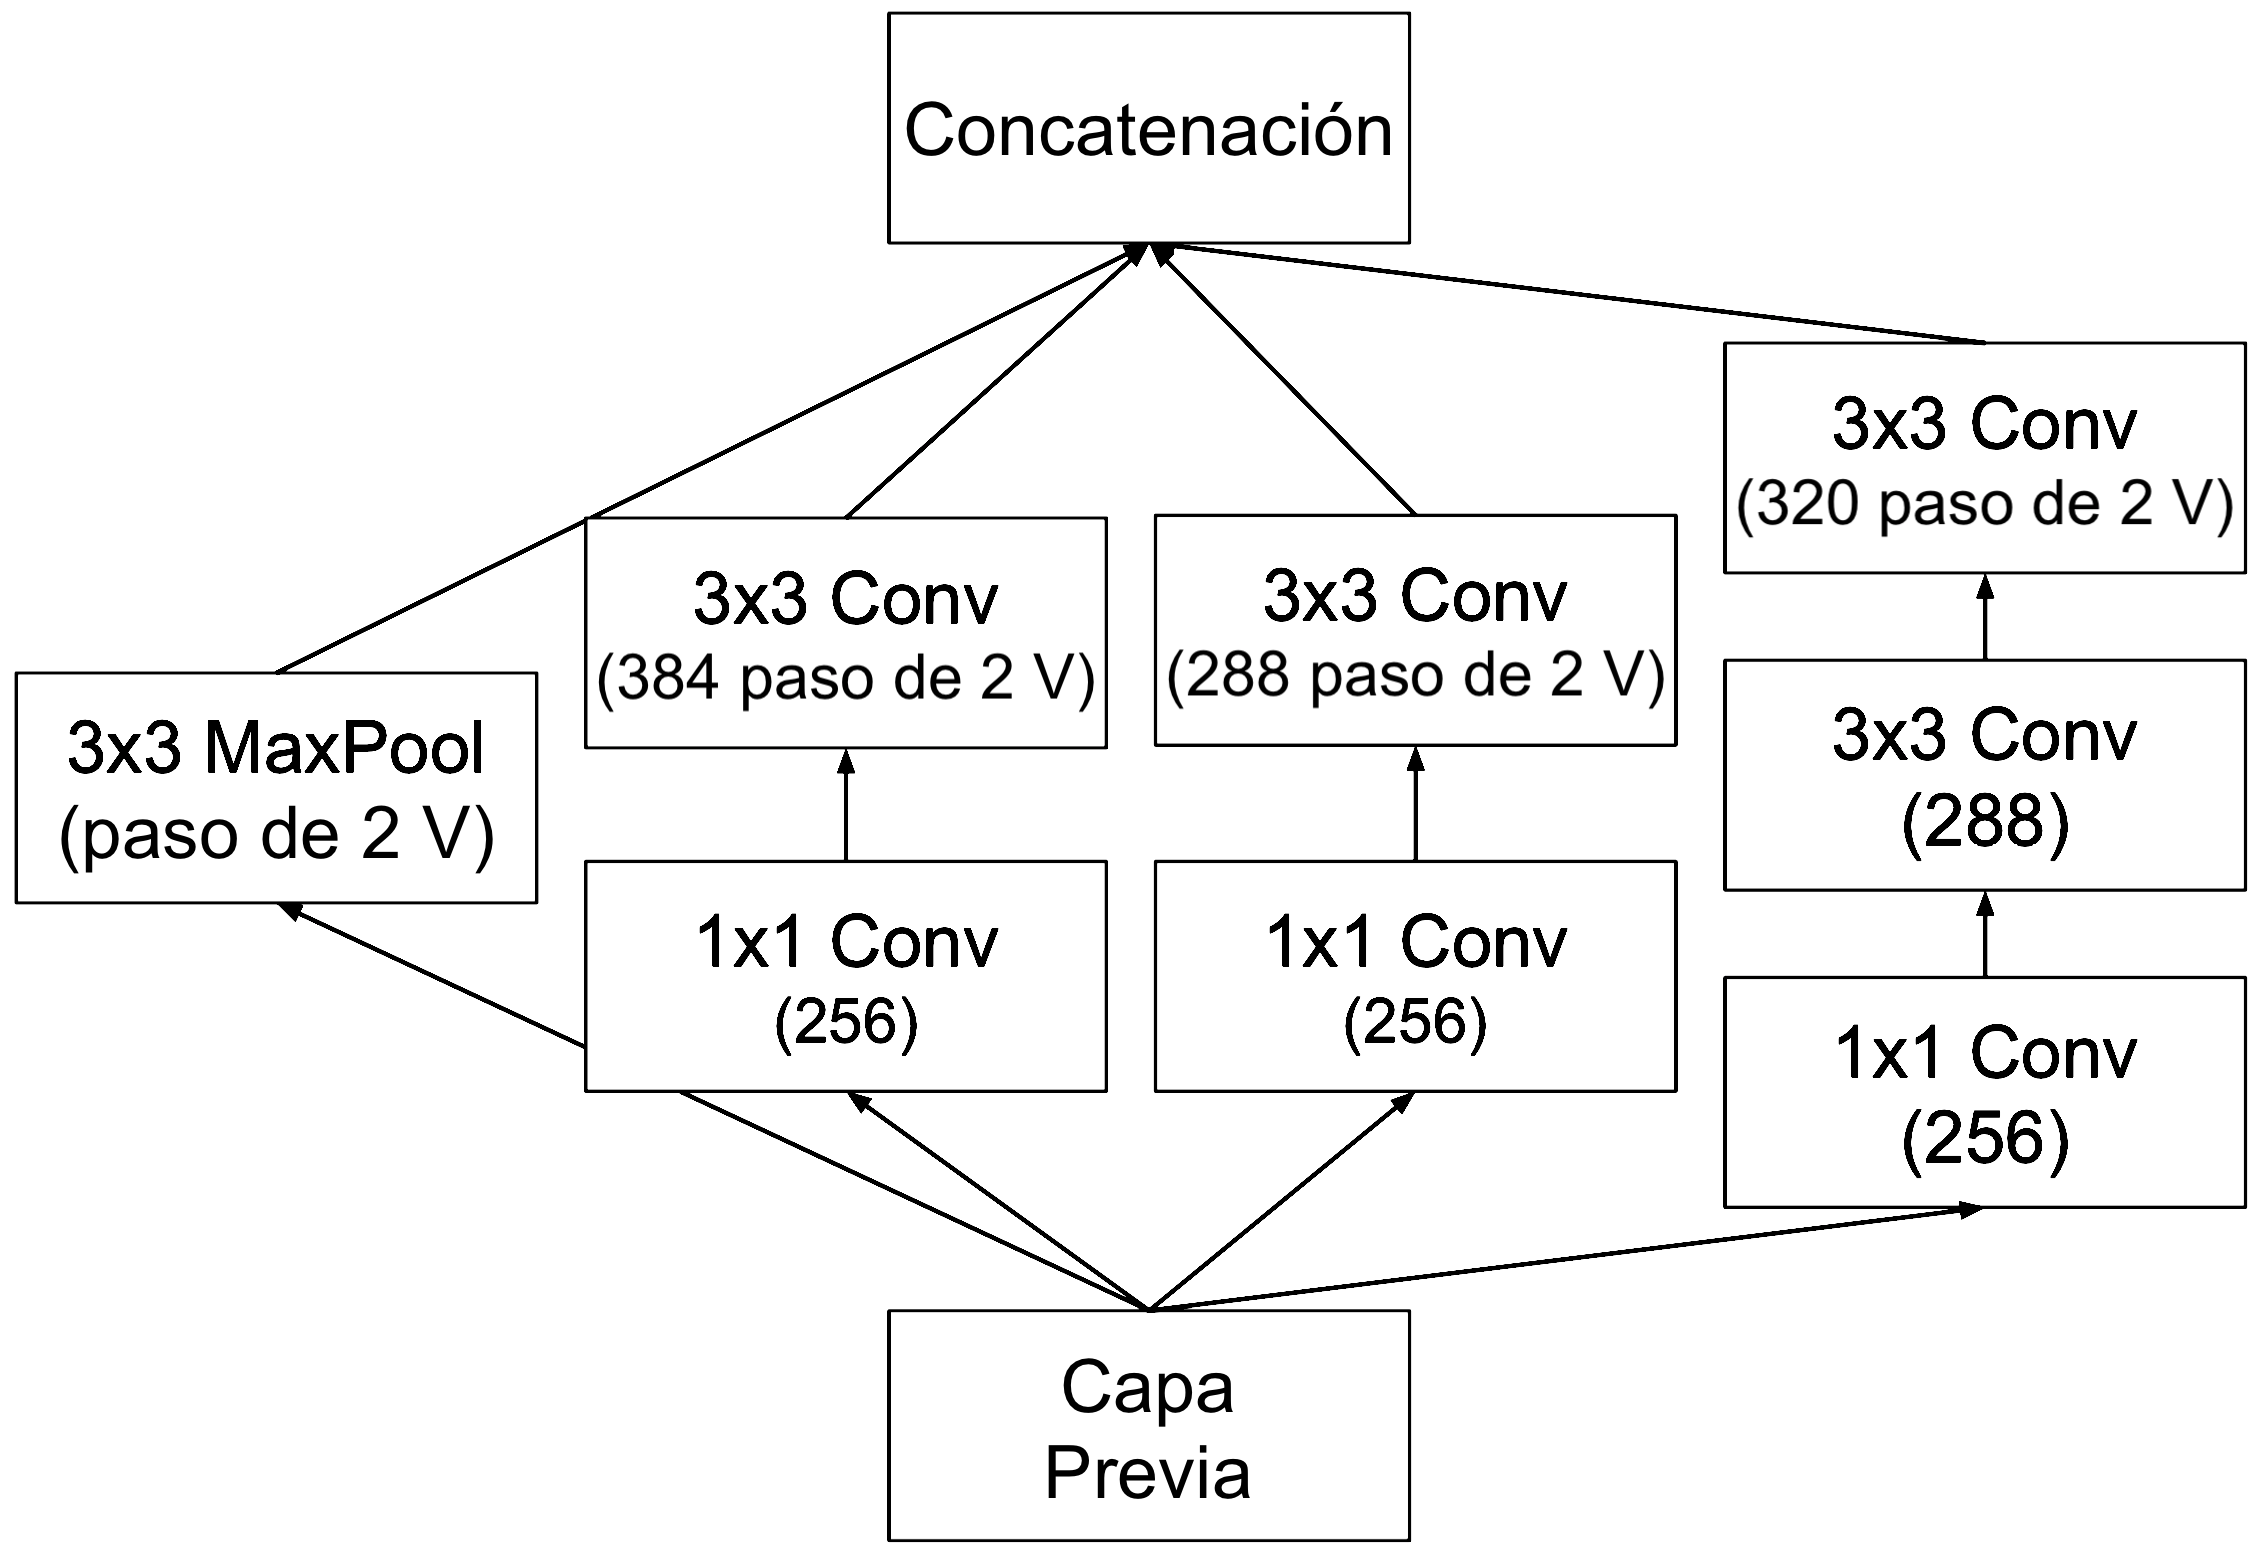
\includegraphics[width=.9\linewidth]{Images/Reduction-B.png}
      \caption{Bloque Reduction-B.}
      \label{fig:Reduction-B}
    \end{subfigure}
    \caption{Módulos empleados en la arquitectura Inception-ResNet-v2 \cite{Inception-ResNet}.}
    \label{fig:Inception-ResNet-v2Modules}
\end{figure}

La arquitectura sintetizada de este modelo se expone en la \autoref{fig:Inception-ResNet-v2}. Como puede observarse, a parte de las estructuras de entrada y de clasificación, cuyo funcionamiento es análogo al descrito en la \autoref{Chapter:ArchitectureInceptionV3}, esta red está formada principalmente por 5 módulos Inception distintos y denominados como Inception-ResNet-A, Reduction-A, Inception-ResNet-B, Reduction-B e Inception-ResNet-C. Estos tipos de bloques, representados en la \autoref{fig:Inception-ResNet-v2Modules}, tienen dos propósitos diferentes, encargándose esencialmente de la construcción de los mapas de características de los datos de entrada y de la reducción de estos espacios de activación con el fin de obtener unas representaciones homólogas de menor tamaño. 

De forma concreta y tras procesarse inicialmente las imágenes en la entrada, esta información es inyectada en los bloques Inception-ResNet-A de la \autoref{fig:Inception-ResNet-A}, que mediante el uso de filtros de dimensiones reducidas ($1\times 1$ y $3\times 3$) son capaces de detectar características muy básicas y disminuir el tamaño de las fotografías. Tras ello, estos datos son introducidos en el módulo Reducción-A expuesto en la \autoref{fig:Reduction-A}, que condensa aún más las dimensiones de las representaciones a fin de acelerar el entrenamiento de los posteriores bloques Inception-ResNet-B de la \autoref{fig:Inception-ResNet-B}. Estos últimos, de hecho, contienen un número menor de capas que sus predecesores Inception-ResNet-A, aunque utilizan filtros de mayor tamaño ($1\times 1$, $1\times 7$ y $7\times 1$) con el propósito de detectar características más complejas. Posteriormente, los resultados de estos últimos módulos son transferidos a la estructura Reduction-B que al contar con más capas que Reduction-A, como puede observarse en la \autoref{fig:Reduction-B}, es capaz de hacer frente a una mayor cantidad de datos que son la consecuencia directa del empleo de filtros de mayores dimensiones en los bloques Inception-ResNet-B. Toda esta información reducida es transferida seguidamente a los módulos Inception-ResNet-C, mostrados en la \autoref{fig:Inception-ResNet-C}, y que debido al aumento de la complejidad de la arquitectura emplean en esta ocasión un número reducido de filtros para aminorar el coste temporal del entrenamiento. Finalmente, la conexión secuencial de todos estos bloques según la \autoref{fig:Inception-ResNet-v2} da lugar a una red con una profundidad considerable, que tras extraer las características de las imágenes inyectadas en la entrada procederá a categorizarlas mediante el módulo clasificador adaptado al contexto del reconocimiento de expresiones faciales y con una arquitectura idéntica a la del modelo Inception-v3.

\subsection{ResNet-50}

\begin{figure}
    \centering
    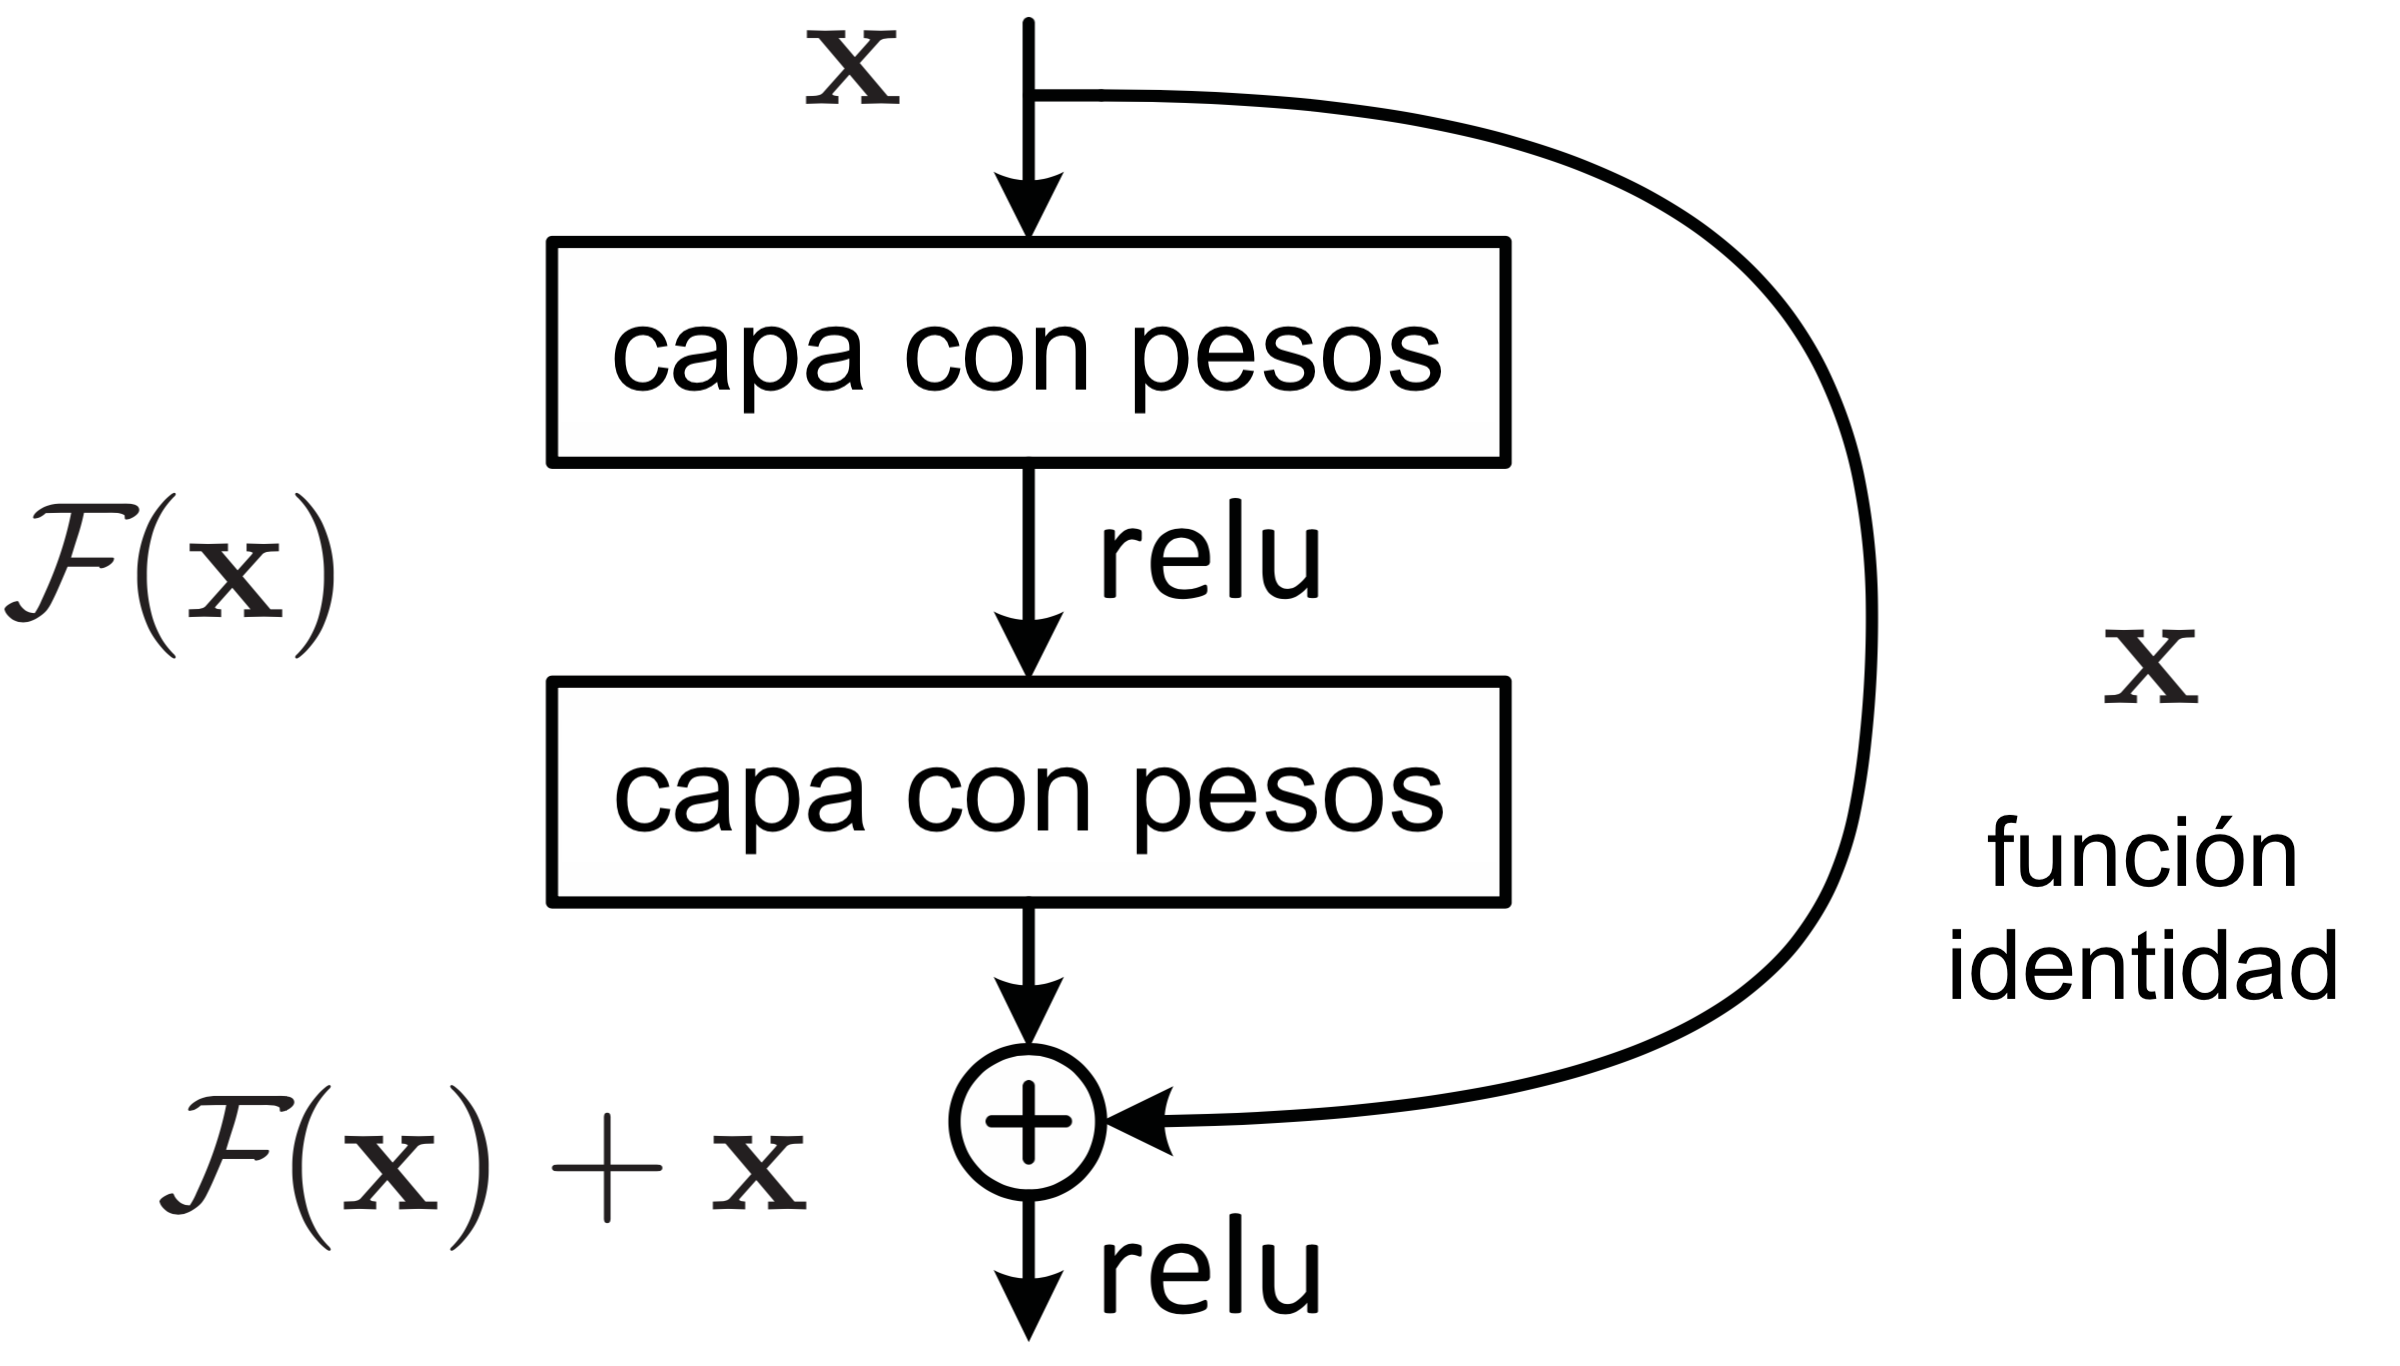
\includegraphics[scale=0.2]{Images/ResnetBlock.png}
    \caption{Bloque residual básico \cite{ResNet}.}
    \label{fig:ResNetBlock}
\end{figure}

La arquitectura ResNet se concibió por primera vez en 2015 \cite{ResNet} como un intento de crear un modelo de clasificación de imágenes que solucionara los problemas de las redes convencionales cuya respuesta, al contrario de lo que se podía intuir, se degradaba significativamente al aumentarse la profundidad. De esta forma, esta investigación demostró que la agregación de ciertas conexiones adicionales que pasaban por alto determinadas capas a las redes tradicionales permitía seguir aumentando el número de niveles sin que el rendimiento decayera. La unidad básica que aprovecha esta idea y de la que se componen este tipo de redes se expone en la \autoref{fig:ResNetBlock}. Como se puede advertir, estos módulos constan básicamente de dos capas convolucionales apiladas y una conexión que agrega los datos de la entrada directamente a la salida, tal y como se muestra en la \autoref{eq:ResNet}.
\begin{align} \label{eq:ResNet}
    H(x) &= F(x) + x \\
    \text{donde}~ 
    x &\equiv \text{entrada del bloque} \notag \\
    F(x) & \equiv \text{función residual aprendida por las dos capas convolucionales} \notag
\end{align}
La hipótesis de esta implementación expone que es más fácil optimizar los coeficientes de la asignación original que se encuentren cerca de la función de identidad forzando la función residual a cero, que realizar un mapeo de identidad mediante una sucesión de capas no lineales \cite{ResNet}. Esta característica es precisamente la que se explota a lo largo de la profundidad de este tipo de redes permitiendo evitar y aliviar cualquier complejidad que vaya apareciendo durante el entrenamiento simplemente mediante la omisión de partes de la red.

\begin{figure}
    \centering
    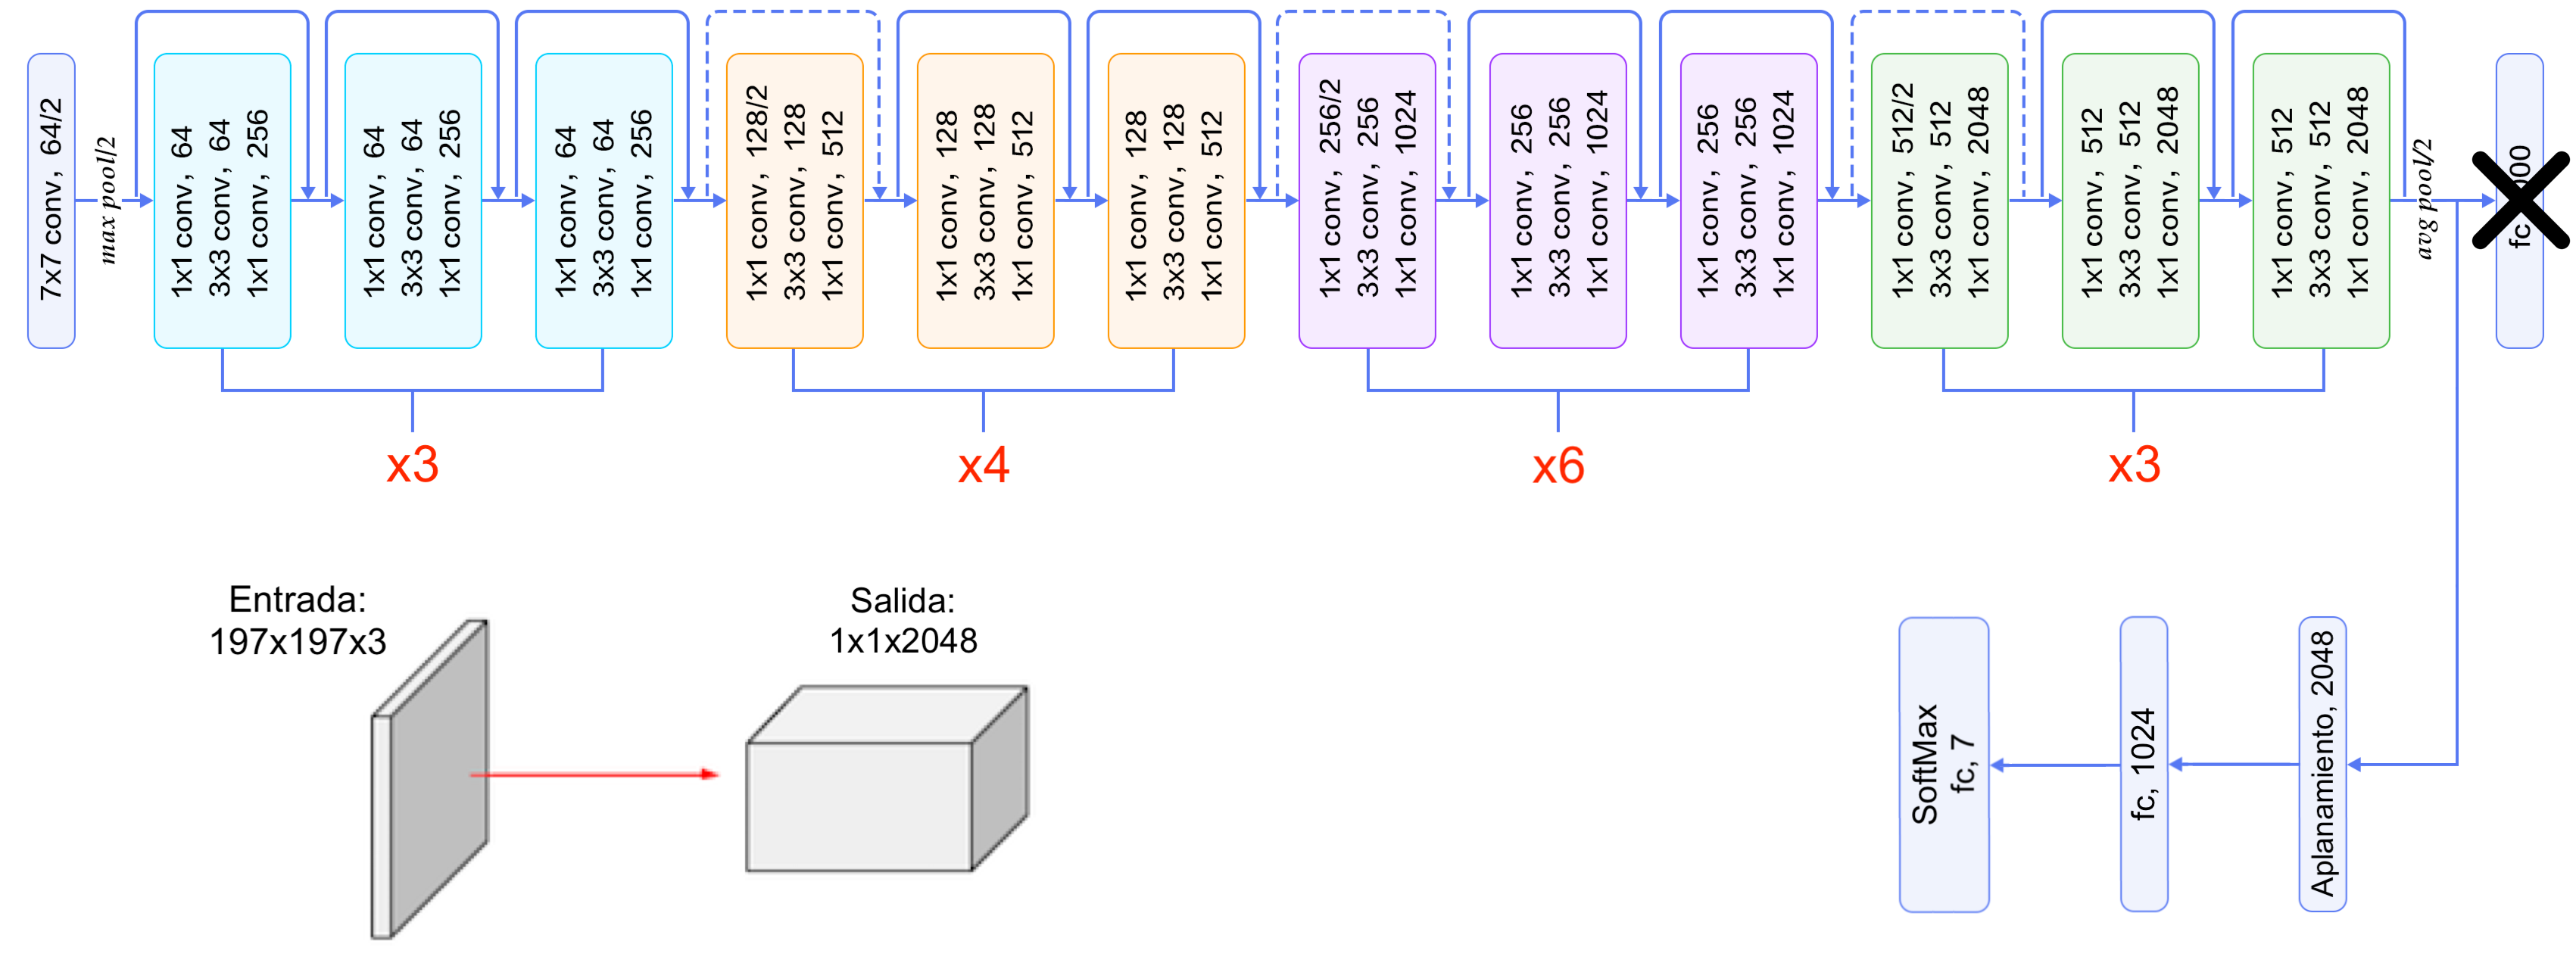
\includegraphics[width=\textwidth]{Images/ResNet-50.png}
    \caption{Arquitectura del modelo ResNet-50 adaptado al problema del reconocimiento de expresiones faciales \cite{img:ResNet-50}.}
    \label{fig:ResNet-50}
\end{figure}

Hay numerosas variaciones de las arquitecturas ResNet, empleándose con una gran variedad de niveles de profundidad (34, 50, 101 e incluso 152 capas). Sin embargo, en el presente proyecto se usa principalmente la ResNet de 50 capas de la \autoref{fig:ResNet-50}, ya que es precisamente la utilizada por el Grupo de Geometría Visual de la universidad de Oxford en el entrenamiento de la base de datos VGGFace2 \cite{VGGFace2} y a partir de cuyos resultados se va a desarrollar la red particular enfocada al problema del reconocimiento de emociones. Como puede observarse, esta arquitectura adaptada no es más que una sucesión de bloques residuales con la novedad, con respecto a los modelos anteriormente descritos, de que, dada la naturaleza de la red, se ha empleado una capa auxiliar de aplanamiento que vincula la etapa de clasificación y la de extracción de características. Asimismo y aunque no aparezcan por simplicidad en la \autoref{fig:ResNet-50}, cabe destacar que son empleadas la capa de activación ReLU y la capa de normalización por lotes en cada una de las etapas convolucionales, tal y como se describió más detalladamente en la \autoref{Chapter:Layers}.

\section{Entrenamiento}

Por un lado, el método de aprendizaje descrito en este apartado trata de aprovechar lo máximo posible las capacidades de la base de datos FER-2013 mediante un preprocesamiento meticuloso y por otro, beneficiarse de los recursos computacionales ofrecidos por la plataforma de Google Cloud.

\subsection{Preprocesamiento de los Datos}

En este proyecto, los objetivos principales del preprocesamiento del conjunto de entrenamiento de la base de datos FER-2013 son el aumento de la heterogeneidad o diversidad de estas imágenes y su adaptación a las características de los distintos modelos empleados, así como a las especificaciones impuestas por ciertas herramientas de la API de Keras. Por todo ello, son aplicadas las siguientes transformaciones a los datos antes de su procesamiento por las arquitecturas planteadas en el apartado anterior:
\begin{itemize}
  \item \textbf{Redimensionamiento}. En primer lugar es necesario modificar la resolución original de $48\times 48$ píxeles de las imágenes del conjunto de datos FER-2013 a las dimensiones aceptadas por los modelos Inception-v3, Inception-ResNet-v2 y ResNet-50 cargados en la librería de Keras. En los tres casos, y dadas las limitaciones de memorias observadas durante el entrenamiento (tratadas más detenidamente en las secciones correspondientes), la conversión se realiza a las proporciones mínimas aceptadas por estas arquitecturas:
        \begin{itemize}
          \item \textbf{Inception-v3}: $139\times 139$ píxeles.
          \item \textbf{Inception-ResNet-v2}: $139\times 139$ píxeles.
          \item \textbf{ResNet-50}: $197\times 197$ píxeles.
        \end{itemize}

  Este proceso se realiza mediante el método considerado como estándar para este tipo de tareas de manipulación de imágenes y es conocido como interpolación bicúbica. A pesar de que su tiempo de procesamiento es más lento en comparación con las alternativas existentes (interpolación bilineal o interpolación por el vecino más cercano) es el que mejor resultados permite obtener en términos de calidad. Por ello y para evitar aumentar más el ruido de las imágenes empleadas, cuya calidad de por sí es bastante pobre, se ha optado por esta opción.
  
  Por otro lado, las tres redes originales presuponen en la entrada imágenes con un modelo de color RGB, por lo que también se hace necesario hacer una conversión de las representaciones de expresiones faciales en escala de grises a esta especificación. Esto es realizado simplemente mediante una reproducción de las imágenes originales a lo largo de las tres dimensiones correspondientes a los tres espacios de color de destino.
  \item \textbf{Normalización}. Dado que tras el redimensionado las imágenes se componen de una serie de coeficientes RGB en el intervalo $[0, 255]$, es indispensable realizar una normalización con el fin de evitar el manejo de valores demasiado altos que generalmente dan lugar a una ralentización del proceso de aprendizaje. Concretamente, y con el objetivo de no eliminar en primera instancia los valores de los pesos iniciales, se han seguido los mismos procedimientos de regularización que los propuestos en las redes originales preentrenadas:
        \begin{itemize}
            \item \textbf{Inception-v3} y \textbf{Inception-ResNet-v2}. Los valores RGB del intervalo $[0, 255]$ son adaptados al espacio $[-1, 1]$ mediante la expresión matemática de la \autoref{eq:PreprocessInception}.
                \begin{align} \label{eq:PreprocessInception}
                  \hat{x} &= \frac{x}{127.5} - 1 & \forall \text{\space} x \in [0, 255]
                \end{align}
            \item \textbf{ResNet-50}: Tanto en el documento original de este modelo \cite{ResNet} como en el artículo que hace uso de la base de datos VGGFace2 \cite{VGGFace2}, la normalización es llevada a cabo mediante la sustracción a cada uno de los píxeles del valor promedio del espacio de color al que corresponden. Mediante este proceso se consigue el centrado de los datos en cero. Sin embargo, dado que el conjunto FER-2013 redimensionado según el punto anterior presenta los mismos coeficientes RGB en los 3 canales, se ha considerado conveniente realizar la sustracción del mismo promedio a cada una de las dimensiones según la \autoref{eq:PreprocessResNet}.
                \begin{align} \label{eq:PreprocessResNet}
                  \hat{x} &= x - \overline{x} = x - 128.8006 & \forall \text{\space} x \in [0, 255]
                \end{align}
            Asimismo, el valor de esta media se ha calculado tan sólo sobre los datos de entrenamiento del conjunto FER-2013, aplicándose posteriormente a los grupos de validación y evaluación. 
        \end{itemize}
        
  \item \textbf{Transformaciones geométricas}. Tal y como se ha visto en la \autoref{Chapter:GeometricTransformations}, la aplicación de una serie de transformaciones geométricas a las imágenes del conjunto de entrenamiento puede enriquecer la base de datos empleada. Por ello, en el caso particular de este proyecto se realizan las siguientes conversiones lineales de forma pseudoaleatoria en cada iteración del entrenamiento:
        \begin{itemize}
          \item \textbf{Rotación}. Es aplicada una rotación de sentido aleatorio de entre 0 y 10 grados sexagesimales a cada una de las imágenes. Para la elección de este valor se han tenido en cuenta el rango máximo de flexión lateral del cuello, que varía entre 20 y 45 grados \cite{LateralFlexion},y el hecho de que ciertas imágenes del conjunto de entrenamiento FER-2013 ya presentan rostros ligeramente girados.
          \item \textbf{Transformación de cizallamiento}. Esta transformación también es conocida como inclinación y es efectuada en las direcciones del eje de abscisas con una intensidad comprendida entre los 0 y los 10 grados sexagesimales.
          \item \textbf{Volteo}. Se fuerza a un volteo horizontal aleatorio de las imágenes inyectadas. 
          \item \textbf{\textit{Zoom}}. A pesar de que los datos de entrenamiento ya se componen de imágenes con rostros centrados y enfocados, se ha recurrido a una ampliación o reducción de carácter aleatorio de las representaciones del 10\% con el objetivo de lograr una mayor generalización.
          \item \textbf{Relleno}. Dado que algunas de las transformaciones anteriormente nombradas implican la introducción de puntos externos a las imágenes en los campos receptivos originales, se hace necesaria la aplicación de un método que evite la inclusión de este ruido. En este contexto se han explorado distintos procedimientos de relleno, como la propagación constante de píxeles o el método de los vecinos más próximos. Sin embargo, los mejores resultados observados experimentalmente se han obtenido mediante la técnica de reflexión de las imágenes transformadas.
        \end{itemize}
\end{itemize}

\subsection{Proceso de Aprendizaje}

El procedimiento llevado a cabo para conseguir un aprendizaje efectivo en cada uno de los modelos ha consistido, en primer lugar, en un entrenamiento tan sólo de las capas de la etapa de clasificación particularizada al problema del reconocimiento de expresiones faciales. Tras esta técnica para evitar una inicialización aleatoria de los niveles superiores se ha seguido con un entrenamiento íntegro de los modelos completos, que es precisamente sobre el cual se van a reportar los resultados finales.

En este contexto, se procede a describir a continuación algunas de las características compartidas del proceso de aprendizaje de los tres modelos descritos anteriormente (Inception-v3, Inception-ResNet-v2 y ResNet-50):
\begin{itemize}
    \item \textbf{Tamaño de los lotes}. Para aprovechar lo máximo posible las capacidades de computo que ofrece la plataforma Google Cloud y agilizar el aprendizaje se consideró oportuno en un primer momento inyectar a los modelos lotes con un número de ejemplos de entrenamiento considerable. Sin embargo, dado que el alimentador de datos provisto por la API de Keras es ejecutado en paralelo al modelo, se ha comprobado experimentalmente que, incluso la GPU más potente ofrecida por Google Cloud (NVIDIA Tesla P100, cuyas características se encuentran en la \autoref{Table:GPU}), es incapaz de asignar la memoria necesaria que requieren los lotes con más de $128$ imágenes. Este problema también es favorecido por la complejidad de los modelos usados, que además presentan una gran cantidad de parámetros como se puede comprobar en la \autoref{Table:Models}, así como por la realización de un intenso preprocesamiento a cada una de las imágenes en cada iteración. Si bien, este último procedimiento está optimizado para que sea realizado exclusivamente por la CPU. Teniendo en cuenta estas consideraciones, se ha llegado a la conclusión de que utilizar lotes de menor tamaño es la manera más simple y efectiva de reducir la memoria demandada. Por todo ello, el tamaño de los lotes se ha estipulado en 128 imágenes. También cabe remarcar que esta dimensión es múltiplo de 2 debido a las evidencias existentes de que de esta manera la GPU es capaz de distribuir de una forma más óptima la carga de trabajo debido a la forma en la que se codifican los datos \cite{BatchSize}.
    \item \textbf{Función de pérdidas}. Hay una gran cantidad de maneras de cuantificar la función de pérdidas que determina la calidad de la predicción realizada con respecto a unos determinados datos de entrada. En el caso particular de este proyecto y considerando la naturaleza de los datos del conjunto FER-2013, categorizados en 7 clases, es empleada la función de la entropía cruzada categórica. Su uso para determinar el desempeño de un modelo concreto en cada iteración está ampliamente extendido y es, de hecho, la elección predeterminada en los problemas de aprendizaje profundo multiclase debido a las mejoras de velocidad que permite obtener con respecto a otras implementaciones tradicionales como el coste cuadrático o el exponencial \cite{CrossEntropy}. Su expresión matemática puede observarse en la \autoref{eq:CrossEntropy}. De esta última también se puede deducir que en el proceso de aprendizaje se intentará minimizar la entropía cruzada entre las probabilidades estimadas y la distribución verdadera, para posteriormente actualizar los pesos correspondientemente.
    \begin{align} \label{eq:CrossEntropy}
        H(p, q) &= \sum\limits_{x} p(x) \log q(x) \\
        \text{donde}~ 
            p(x) &\equiv \text{distribución verdadera donde toda la masa de probabilidad está en la clase} \notag \\
               & \text{ correcta, es decir, $p = [0, ... 1, ..., 0]$ contiene un único $1$ en la posición iésima} \notag \\
            q(x) & \equiv \text{distribución estimada} \notag
    \end{align}
    \item \textbf{Iteraciones de entrenamiento de las capas superiores}. Dado que el objetivo del entrenamiento de la etapa de clasificación introducida es la obtención de unos resultados ligeramente superiores a los obtenidos con la inicialización aleatoria, que ajusta los pesos iniciales con una distribución uniforme en el intervalo $[-0.05, 0.05]$, se ha estipulado un número de tan sólo 5 iteraciones, que ha permitido alcanzar tasas de acierto en esta subred de entre el 20\% y el 30\%.
    \item \textbf{Optimizador empleado en el entrenamiento de las capas superiores}. En la práctica, el optimizador Adam es recomendado como el algoritmo predeterminado para las tareas de aprendizaje profundo ya que su uso requiere un menor número de iteraciones para converger que la alternativa SGD y sus variantes \cite{CS231n}. Sin embargo, este optimizador es propenso en algunas ocasiones a no alcanzar la convergencia más óptima \cite{AdamToSDG}, aunque dado que la etapa de clasificación introducida tan sólo se va a entrenar durante 5 iteraciones en este punto, este hecho carece de importancia. Los parámetros utilizados son los especificados por defecto en el artículo que describe este algoritmo \cite{Adam} y cuya notación está vinculada a lo descrito en la \autoref{Chapter:Adam} y concretamente a la \autoref{eq:Adam}: $\lambda = 0.001, \beta_1 = 0.9, \beta_2 = 0.999, \epsilon = 10^{-8}$.
    \item \textbf{Iteraciones de entrenamiento del modelo completo}. Los tres modelos tienen especificado un entrenamiento de 100 iteraciones sobre la arquitectura completa, aunque tal y como se verá a continuación se ha considerado conveniente interrumpir el proceso de aprendizaje en el momento en el que vayan apareciendo indicios de convergencia con el propósito de no consumir recursos de forma innecesaria.
\end{itemize}

En lo que respecta al entrenamiento de la red completa, a lo largo del entrenamiento de los sucesivos modelos se han ido explorando y ajustando ciertos parámetros que se procederán a describir a continuación.

\subsubsection{Inception-v3 e Inception-ResNet-v2}

Dado que estos dos modeles han sido preentrenados con la base de datos ImageNet, que como se vio en la \autoref{Chapter:ImageNet} difiere en gran medida del conjunto FER-2013 empleado en este proyecto, se procederá a afinar los pesos de todas las capas originales ya que es probable que incluso en los niveles inferiores la red extraiga características no relevantes para la tarea del reconocimiento de expresiones faciales.

En lo que respecta al proceso de aprendizaje en sí, para la actualización de los pesos de la red completa del modelo Inception-v3 se ha considerado oportuno utilizar el optimizador SGD con Nesterov Momentum puesto que Adam suele lograr una generalización peor para los conjuntos de validación y evaluación \cite{AdamToSDG}. De igual manera, es usada una tasa de aprendizaje más pequeña que la especificada por defecto con la intención de no distorsionar los pesos iniciales demasiado rápido y más cuando el clasificador introducido está siendo entrenado a partir de una inicialización incierta. En consecuencia, son elegidos una tasa de aprendizaje de $\lambda = 10^{-4}$ y un momento lineal de $\mu = 0.9$ \cite{Sutskever} siguiendo la notación de la \autoref{eq:SGDNM_1}.

A pesar de todo ello, al ser los resultados del modelo Inception-v3 no del todo satisfactorios, tal y como se comprobará en la \autoref{Chapter:Results}, se ha tomado la decisión de entrenar un tipo de red más compleja, como es Inception-ResNet-v2, y con una tasa de aprendizaje inicial más agresiva de $\lambda = 0.001$ para optimizar los tiempos de entrenamiento y de convergencia. Sin embargo, dado que el empleo de tasas de aprendizaje altas conlleva el riesgo de estancamiento en peores valores de pérdidas, también se ha considerado conveniente ir disminuyendo la tasa de aprendizaje a la mitad cada 5 iteraciones.

Asimismo, en las dos implementaciones y para tener un control adicional sobre el proceso de entrenamiento en caso de que el modelo alcance la convergencia o se quede estancado en algún punto, se ha introducido una función que disminuye la tasa de aprendizaje a la mitad si no se obtiene ninguna mejora del valor de pérdidas durante 5 iteraciones seguidas en el caso de Inception-v3 y de 3 en el caso de Inception-ResNet-v2. De igual manera, se ha estipulado que se detenga completamente el entrenamiento y se guarde el contexto si las pérdidas no son reducida durante 20 iteraciones seguidas durante el proceso de aprendizaje del modelo Inception-v3 y durante 10 iteraciones en el caso de la red Inception-ResNet-v2.

\subsubsection{ResNet-50}

En esta ocasión la base de datos VGGFace2 expuesta en la \autoref{Chapter:VGGFace2} y empleada por esta red sí que presenta una gran similitud con el conjunto FER-2013, por lo que es posible suponer que al menos los primeros niveles van a extraer características de interés para el problema del reconocimiento de emociones. Por este motivo y teniendo en cuenta las limitaciones de tamaño que presenta el conjunto FER-2013, se ha decidido dejar los pesos de los primeros 6 módulos residuales (los módulos de color azul de la \autoref{fig:ResNet-50}) sin afinar para evitar el sobreaprendizaje del modelo. El resto de bloques ha sido entrenado con normalidad y empleando, al igual que en los modelos anteriores, un optimizador SGD con Nesterov Momentum con los siguientes parámetros: $\lambda = 10^{-4}$ y $\mu = 0.9$. También es necesario señalar que se ha estipulado que esta tasa de aprendizaje, $\lambda$, se reduzca a la mitad cada vez que el desempeño del modelo, en lo que respecta a las pérdidas, no mejore durante 3 iteraciones seguidas, interrumpiéndose el entrenamiento completamente a las 10 iteraciones de no presentar avances.

Finalmente cabe destacar que tanto en este modelo como en los anteriores se hace un seguimiento del proceso de aprendizaje en tiempo real mediante la utilización de la herramienta Tensorboard ofrecida por TensorFlow y que permite exportar y representar gráficamente desde Keras ciertas métricas cuantitativas. En el caso particular de este proyecto se monitorizan las tasas de pérdidas y de acierto sobre los datos de entrenamiento y validación y la tasa de aprendizaje. Del mismo modo, también se van guardando los puntos de control del mejor modelo obtenido hasta la fecha en cada iteración del entrenamiento.

\subsection{Despliegue en la Plataforma Google Cloud}

Para realizar el entrenamiento de los modelos Inception-v3, Inception-ResNet-v2 y ResNet-50 se ha empleado la herramienta descrita en la \autoref{Chapter:GoogleCloud} y conocida como Cloud Datalab. El motivo detrás de esta decisión es que este servicio es precisamente el que permite un despliegue más inmediato de los modelos al emular el funcionamiento de los \textit{notebooks} de Python y la que ofrece la GPU con las mejores características en términos de desempeño y memoria (NVIDIA Tesla P100). De hecho, el empleo de la herramienta alternativa (Cloud Machine Learning Engine) implica una reducción excesiva del tamaño de los lotes, lo que no favorece para nada el tiempo de entrenamiento, al ofrecer tan sólo los servicios de la GPU NVIDIA Tesla K80, con un tamaño de memoria que es la mitad que la de la GPU NVIDIA Tesla P100.

\section{Resultados} \label{Chapter:Results}

\begin{table}
    \centering
    \begin{tabular}{c|c|c|c|c|c|}
    \cline{2-6}
    & \textbf{\begin{tabular}[c]{@{}c@{}}Tasa de\\ acierto\end{tabular}} & \textbf{\begin{tabular}[c]{@{}c@{}}Tiempo de\\ entrenamiento\end{tabular}} & \textbf{Iteraciones} & \textbf{\begin{tabular}[c]{@{}c@{}}Número de\\ parámetros\end{tabular}} & \textbf{\begin{tabular}[c]{@{}c@{}}Tamaño del\\ modelo\end{tabular}} \\ \hline
    \multicolumn{1}{|c|}{\textbf{Inception-v3}} & 0.6386 & 5h 9m 37s & 80 & 23\,873\,703 & 192.1 MB \\ \hline
    \multicolumn{1}{|c|}{\textbf{Inception-ResNet-v2}} & 0.6500 & 1h 4m 26s & 27 & 55\,857\,255 & 449.3 MB \\ \hline
    \multicolumn{1}{|c|}{\textbf{ResNet-50}} & 0.7125 & 2h 29m 45s & 40 & 25\,613\,383 & 308.3 MB \\ \hline
    \end{tabular}
\caption{Comparación entre las características de los distintos modelos empleados y su desempeño sobre el conjunto de evaluación de la base de datos FER-2013.}
\label{Table:Models}
\end{table}


Los resultados de los entrenamientos se encuentran sintetizados en la \autoref{Table:Models}. 



\begin{table}[]
\centering
\caption{My caption}
\label{my-label}
\begin{tabular}{c|c|c|c|c|c|}
\cline{2-6}
 & \textbf{\begin{tabular}[c]{@{}c@{}}Tasa de\\ acierto\end{tabular}} & \textbf{\begin{tabular}[c]{@{}c@{}}Tiempo de\\ entrenamiento\end{tabular}} & \textbf{\begin{tabular}[c]{@{}c@{}}Iteraciones de\\ entrenamiento\end{tabular}} & \textbf{\begin{tabular}[c]{@{}c@{}}Número de\\ parámetros\end{tabular}} & \textbf{\begin{tabular}[c]{@{}c@{}}Tamaño del\\ modelo\end{tabular}} \\ \hline
\multicolumn{1}{|c|}{\textbf{Inception-v3}} & 0.6386 & 5h 9m 37s & 80 & 23,873,703 & 192.1 MB \\ \hline
\multicolumn{1}{|c|}{\textbf{Inception-ResNet-v2}} & 0.6500 & 1h 4m 26s & 27 & 55,857,255 & 449.3 MB \\ \hline
\multicolumn{1}{|c|}{\textbf{ResNet-50}} & 0.7125 & 2h 29m 45s & 40 & 25,613,383 & 308.3 MB \\ \hline
\end{tabular}
\end{table}


\subsection{Inception-v3}

\cite{Inception-v3}

\subsection{Inception-ResNet-v2}


\cite{Inception-ResNet}


\subsection{ResNet-50}

\cite{ResNet}





